% options:
% thesis=B bachelor's thesis
% thesis=M master's thesis
% czech thesis in Czech language
% slovak thesis in Slovak language
% english thesis in English language
% hidelinks remove colour boxes around hyperlinks

\documentclass[thesis=M,czech]{FITthesis}[2012/06/26]

\usepackage[utf8]{inputenc} % LaTeX source encoded as UTF-8

\usepackage{graphicx} %graphics files inclusion
% \usepackage{amsmath} %advanced maths
% \usepackage{amssymb} %additional math symbols

\usepackage{dirtree} %directory tree visualisation

\usepackage{scrextend}
\usepackage{listings}
\usepackage{color}
 
\definecolor{dkgreen}{rgb}{0,0.6,0}
\definecolor{gray}{rgb}{0.5,0.5,0.5}
\definecolor{mauve}{rgb}{0.58,0,0.82}
\definecolor{gray}{rgb}{0.4,0.4,0.4}
\definecolor{darkblue}{rgb}{0.0,0.0,0.6}
\definecolor{lightblue}{rgb}{0.0,0.0,0.9}
\definecolor{cyan}{rgb}{0.0,0.6,0.6}
\definecolor{darkred}{rgb}{0.6,0.0,0.0}


\lstset{
  basicstyle=\ttfamily\footnotesize,
  columns=fullflexible,
  showstringspaces=false,
%  numbers=left,                   % where to put the line-numbers
%  numberstyle=\tiny\color{gray},  % the style that is used for the line-numbers
%  stepnumber=1,
%  numbersep=5pt,                  % how far the line-numbers are from the code
  backgroundcolor=\color{white},      % choose the background color. You must add \usepackage{color}
  showspaces=false,               % show spaces adding particular underscores
  showstringspaces=false,         % underline spaces within strings
  showtabs=false,                 % show tabs within strings adding particular underscores
  frame=single,                   % adds a frame around the code
  rulecolor=\color{black},        % if not set, the frame-color may be changed on line-breaks within not-black text (e.g. commens (green here))
  tabsize=2,                      % sets default tabsize to 2 spaces
  captionpos=b,                   % sets the caption-position to bottom
  breaklines=true,                % sets automatic line breaking
  breakatwhitespace=false,        % sets if automatic breaks should only happen at whitespace
  title=\lstname,                   % show the filename of files included with \lstinputlisting;
                                  % also try caption instead of title  
  commentstyle=\color{gray}\upshape
}


\lstdefinelanguage{XML}
{
  morestring=[s][\color{mauve}]{"}{"},
  morestring=[s][\color{black}]{>}{<},
  morecomment=[s]{<?}{?>},
  morecomment=[s][\color{dkgreen}]{<!--}{-->},
  stringstyle=\color{black},
  identifierstyle=\color{lightblue},
  keywordstyle=\color{red},
  morekeywords={xmlns,xsi,noNamespaceSchemaLocation,type,id,x,y,source,target,version,tool,transRef,roleRef,class,name}% list your attributes here
} %syntax highlighting for XML

% % list of acronyms
% \usepackage[acronym,nonumberlist,toc,numberedsection=autolabel]{glossaries}
% \iflanguage{czech}{\renewcommand*{\acronymname}{Seznam pou{\v z}it{\' y}ch zkratek}}{}
% \makeglossaries

\newcommand{\tg}{\mathop{\mathrm{tg}}} %cesky tangens
\newcommand{\cotg}{\mathop{\mathrm{cotg}}} %cesky cotangens

% % % % % % % % % % % % % % % % % % % % % % % % % % % % % % 
% ODTUD DAL VSE ZMENTE
% % % % % % % % % % % % % % % % % % % % % % % % % % % % % % 

\department{Katedra softwarového inženýrství}
\title{Children Usability Lab - management video streamů}
\authorGN{Patrik} %(křestní) jméno (jména) autora
\authorFN{Faistaver} %příjmení autora
\authorWithDegrees{Bc. Patrik Faistaver} %jméno autora včetně současných akademických titulů
\supervisor{Ing. Jiří Chludil}
\acknowledgements{Rád bych poděkoval vedoucímu mé diplomové práce Ing. Jiřímu Chludilovi i oponentovi Ing. Jiřímu Melnikovovi za užitečné připomínky a mnoho cenných rad. Dále chci poděkovat své rodině a blízkým přátelům za podporu a motivaci při tvorbě této práce i během celého studia.}
\abstractCS{Tato diplomová práce navazuje na bakalářskou práci Karolíny Solanské s názvem Children Usability Lab - aplikace pro správu laboratoře. Její bakalářská práce je zde rozšířena o návrh a implementaci subsystému pro management veškerých záznamů nahrávaných v laboratoři Children Usability Lab. Součástí této práce je také analýza současného systému i existujících řešení pro požadovanou správu záznamů, dále pak návrh, realizace a její následné testování. Implementované rozšíření stávajícího systému plně pokrývá dohodnuté zadání i specifikované požadavky.
\par
Závěrem této diplomové práce je podrobení subsystému integračním i akceptačním testům. Subsystém se podařilo úspěšně nasadit do počítačového prostředí laboratoře Children Usability Lab, kde usnadňuje a zefektivňuje tamní usability testování.}

\abstractEN{Sem doplňte ekvivalent abstraktu Vaší práce v~angličtině.}
\placeForDeclarationOfAuthenticity{V~Praze}
\declarationOfAuthenticityOption{4} %volba Prohlášení (číslo 1-6)
\keywordsCS{testování použitelnosti, webová aplikace, laborator uživatelského testování, management záznamů, správa videa}
\keywordsEN{Nahraďte seznamem klíčových slov v angličtině oddělených čárkou.}

\begin{document}

% \newacronym{CVUT}{{\v C}VUT}{{\v C}esk{\' e} vysok{\' e} u{\v c}en{\' i} technick{\' e} v Praze}
% \newacronym{FIT}{FIT}{Fakulta informa{\v c}n{\' i}ch technologi{\' i}}

\begin{introduction}
Testování použitelnosti je proces při kterém se aplikace testuje přímo za pomocí vzorku koncových uživatelů a díky kterému 
se autoři aplikace dozvědí, jak jsou různé prvky uživatelského rozhraní srozumitelné a jak dobře jsou uživatelé schopni se v aplikaci orientovat. V současném světě technologií tento proces vyžaduje informační systém jako řešení pro usnadnění testování, plánování i komunikace mezi jednotlivými subjekty v laboratoři testování použitelnosti. Vývoj takovéhoto systému byl zahájen bakalářskou prací Karolíny Solanské s názvem Children Usability Lab - aplikace pro správu laboratoře (odkazem \cite{solankar}). Její práce vyvinula systém, který slouží jako webová aplikace zajišťující plánování a organizaci testů použitelnosti. Zmíněná bakalářská práce měla neobvykle větší počet stran, avšak podařilo se implementovat zcela funkční systém, ale i přesto je v něm spoustu možností pro vyvinutí nových funkcí. Na tomto základě se dá říci, že se jedná o celkem rozsáhlý systém. Jeden ze směrů, kterým by se systém mohl začít rozšiřovat byla veškerá práce s videem což bylo ostatně zmíněno v uvedené práci v kapitole o dalším vývoji.

Laboratoř použitelnosti na Fakultě informačních technologií ČVUT v Praze je vybavena spoustou zařízení, která jsou schopná zaznamenávat různorodá data. Jedná se nejen o všechna výpočetní zařízení, na kterých probíhají samotné testy, jako hlavní stolní počítač, tablet apod., ale také spousta kamer, mikrofonů či dokonce snímač pohybu očí po obrazovce. Není pochyb o tom, že data z těchto nahrávání schopných zařízení mohou značně přispět ke zkvalitnění vyhodnocování testů použitelnosti. V aktuálním stavu je práce se záznamy velice obtížná a neúčinná, jak je uvedeno v kapitole o současném stavu (\ref{sec:analyza_predchozi_prace}). Z těchto důvodů je nutné rozšířit stávající systém o funkcionalitu, která práci s těmito záznamy značně ulehčí a zefektivní. Jedná se o to, aby uživatelé systému mohli jednoduše pouze přes webové rozhraní spustit a zastavit nahrávání z vybraných zařízení, záznamy roztřídit, uložit v požadovaném formátu a kompresi, upravovat zadaným výčtem způsobů, posílat přes síť do systému SAGE a podobně.
\end{introduction}

\chapter{Cíl práce}
Cílem této diplomové práce je nejprve seznámení se s bakalářskou prací Karolíny Solanské s názvem Children Usability Lab - aplikace pro správu laboratoře (\cite{solankar}). V uvedené práci je třeba analyzovat veškeré specifické požadavky zaměřené na správu videa. Tyto požadavky je nutné znovu probrat s koordinátory  laboratoře Children Usability Lab, aktualizovat je a zakomponovat do specifických požadavků této práce. Vedle převzatých požadavků se nadefinuje i spousta dalších, nových funkčních i nefunkčních požadavků, které byly nashromážděny během posledních let běhu testů v laboratoři. Další částí analýzy je pak ponoření se do světa technologií, které usnadňují práci s videem a z existujících je třeba vybrat pokud možno ty nejvhodnější, které by se daly použít v praktické části této práce.
	
	Výstup analytické části si poté převezme návrhová a implementační část, ve kterých se pomocí nástrojů softwarového inženýrství promění nabyté poznatky v reálný produkt, tedy modul pro správu videa, který půjde se stávajícím systémem provázat.
	
	Se vzniklým testovatelným řešením se pak postoupí do testovací části, kde se otestují funkčnosti zadané specifikací, provede se nasazení, případné opravy nalezených chyb a dále akceptační testování.
Součástí práce bude také dokumentace včetně instalační příručky pomocí které bude možné systém nasadit v různých laboratořích pro testování použitelnosti.

\chapter{Analýza}

\section{Definice pojmů} \label{sec:analyza_definice_pojmu}
\textbf{Frontend}\\
Jedná se o část aplikace, která je viditelná běžným uživatelům.\\ \\
\textbf{Backend}\\
Jedná se o část aplikace, uživatelům \uv{schovaná} za frontendem a slouží především ke zpracování dat.\\ \\
\textbf{CHUL}\\
Children Usability Lab - labratoř testování použirelnosti na Fakultě informačních technologií ČVUT v Praze.\\ \\
\textbf{CDN}\\
CDN neboli Content Delivery Network je systém serverů rozmístěných po internetu, které spolupracují pro zajištění rychlého doručení dat klientovi.\\ \\
\textbf{Hosting}\\
Pronájem úložného prostoru uživateli na proprietárních serverech.\\ \\
\textbf{Framework}\\
Jedná se o softwarovou strukturu fungující jako knihovna funkcí a podpůrných nástrojů, která usnadňuje vývoj jiných softwarových projektů.\\ \\
% \textbf{}\\
% TODO.\\ \\

\section{Rozbor zadání} \label{sec:analyza_rozbor_zadani}
\begin{enumerate}
	\item \textbf{Analyzujte a aktualizujte funkční i nefunkční požadavky zaměřené na správu videa, uvedené v předchozí
práci.\\}
	Jak již bylo zmíněno, tak tato práce navazuje na bakalářskou práci Karolíny Solanské s názvem Children Usability Lab - aplikace pro správu laboratoře (odkazem \cite{solankar}). Aby navázání na předchozí práci mělo ten správný směr, je nutné analyzovat specifické požadavky z předchozí práce, ty projednat s aktuálním vedoucím práce, aktualizovat jejich znění a zařadit do specifických požadavků této práce. Náplň tohoto kroku zadání je detailněji probrána v sekci zabývající se požadavky předchozí práce (vizte \ref{subsec:analyza_predchozi_prace_pozadavky}) a také v sekci s definicí specifických požadavků této práce (\ref{subsec:analyza_fp}).
	\item \textbf{Analyzujte nástroje pro zpracování videa použitelné v infrastruktuře SAGE.\\}
	Většinová část této práce se týká zpracování videa, proto je nezbytně nutné se s oblastí zpracování videa důkladně seznámit. 
	Nejprve je nutné si stanovit, co se bude po pomocných technologiích chtít, tedy seznam obecných funkcí a vlastností a jejich priorit. Na základě tohoto seznamu je třeba provést rešerši existujících technologií a pak všechny nashromážděné poznatky je třeba využít v porovnávací metodice pomocí které se vyberou ty nejvhodnější technologie. Rešerší existujících technologií a různých řešení se zabývá podkapitola o existujících komplexních řešeních (\ref{sec:analyza_existujici_reseni}) a to, které technologie byly zvoleny je podrobně shrnuto v podkapitole o vybraných technologiích (\ref{sec:analyza_technologie}).
	\item \textbf{Pomocí nástrojů a metod softwarového inženýrství navrhněte rozšíření stávající aplikace o moduly pro
správu videa s následující funkcionalitou: přenos po síti včetně ukládání, střih dle zadaných parametrů,
změna rozlišení, možnost komprese, editace meta-informací, transformace obrazu atd.\\}
	Tím nejzajímavějším bodem zadání je právě návrh zadaného řešení. V kapitole o návrhu (\ref{chap:navrh}) se jedná především o sloučení poznatků nabytých v analýze se znalostmi softwarového návrhu. Za užití nástrojů a metod softwarového inženýrství je proveden návrh frontendové i backendové části řešení. Pro moduly zajišťující jednotlivé typy úprav videa je využito technologií studovaných v analytické kapitole(vizte \ref{sec:analyza_technologie}).  
	\item \textbf{Implementujte zmíněné rozšíření stávající aplikace (schopné kooperace s aplikací pro správu laboratoře
CHUL).\\}
	V této produktivní části je na základě návrhu implementován prototyp rozšíření stávající aplikace se všemi zadanými funkcionalitami. Výstupem implementace je pak produkt splňující specifikované požadavky alespoň rámcově, ale zároveň tak, aby bylo možné jej začít testovat a v případě nalezení chyb je opravovat.  
	\item \textbf{Aplikaci podrobte integračním a akceptačním testům.\\}
	Tímto bodem se zabývá celá kapitola o testování (vizte \ref{chap:testovani}), ve které se provedou nejprve zmíněné integrační testy, kterými se ověří bezchybná komunikace mezi jednotlivými komponentami uvnitř rozšíření stávající aplikace. V poslední řadě se provedou akceptační testy právě v CHUL laboratoři.
\end{enumerate}

\section{Předchozí práce a aktuální stav} \label{sec:analyza_predchozi_prace}
Jak bylo řečeno v úvodu, bakalářská práce Karolíny Solanské vyvinula systém, který slouží jako webová aplikace zajišťující plánování a organizaci testů použitelnosti. Tento systém byl vytvořen jako plně funkční vůči zadaným požadavkům a je nasazen v laboratoři CHUL. 
	Systém je celý implementován v jazyku PHP s použitím frameworku Nette. Systém je nasazený na externím serveru s přístupem přes protokoly HTTP a HTTPS. Technologie pro použitou databázi je PostgreSQL.
	Aktuální stav správy videa je příliš nepohodlný a zdlouhavý. Webová aplikace nijak nekomunikuje s jakýmkoliv zařízením v laboratoři CHUL. Vše okolo videí se tedy musí dělat víceméně ručně. V tomto kontextu se pracuje s úžasnou knihovnou \textit{libyuri}(vizte \cite{yuri}), která za pomocí dvou konfiguračních souborů spustí nahrávání, sloučí obrazy a zvuk, uloží a případně zobrazí v systému SAGE. Naneštěstí existují pouze tyto 2 konfigurace, které se ještě ke všemu musí ručně pouštět z příkazové řádky. Nyní neexistuje žádná jednoduchá možnost, jak pohodlně pracovat se záznamy (například ořezávat, přidávat titulek apod.) a tím se tedy bude zabývat tato práce.
	
\subsection{Požadavky předchozí práce} \label{subsec:analyza_predchozi_prace_pozadavky}
Zde jsou uvedeny všechny funkční požadavky z předchozí práce, zaměřené na správu videa a které podpořily důvod vzniku této práce.
\begin{enumerate}
	\item \textbf{Systém ke každému scénáři po proběhlém testu připojí video/videa.\\}
Před začátkem testu si moderátor zvolí scénář a testera, který test provádí. Následně zvolí spuštění testu a test začne. Po dokončení scénáře pak moderátor zvolí ukončení testu. Systém si zaznamená čas a dle toho připojí k jednotlivými experimentům výsek videa odpovídající časovým značkám začátku a konce experimentu.

	\item \textbf{Moderátor a zadavatel mohou video přehrávat, zastavit a převíjet.\\}
Webové grafické rozhraní bude umožňovat zobrazení náhledu videa, které bude fungovat, jako jednoduchý video přehrávač.

	\item \textbf{Moderátor a zadavatel mohou pořídit screenshot videa a okomentovat ho, následně uložit k danému testu.\\}
Bude možné vybrat konkrétní snímek videa (v rámci sekund), ten okomentovat a uložit k danému testu. K testu bude možné přiložit několik snímků (kde každý snímek bude vždy možné utvořit pouze z videí od daného testu).

	\item \textbf{Moderátor a zadavatel mohou video exportovat a stáhnout.\\}
Moderátor a zadavatel mohou video vyexportovat v několika různých formátech. Možné je stažení videa, ale také umístění na server YouTube.

	\item \textbf{Moderátor a zadavatel mohou video konvertovat.\\}
Moderátor a zadavatel mají možnost video převést na jiný formát, především pro kompatibilitu s různými zařízeními a prohlížeči.

	\item \textbf{Moderátor může k videu nahrát mluvený komentář.\\}
Uživatel bude moci nahrát zvuk k libovolnému videu ze vstupního zařízení.
\end{enumerate}

\section{Specifikace požadavků} \label{sec:analyza_pozadavky}
\subsection{Funkční požadavky} \label{subsec:analyza_fp}
\begin{description}
  \item \textbf{F1 -- Nahrávání záznamů}
  \begin{description}
    \item \textbf{F1.1 -- Zobrazení seznamu připojených nahrávacích zařízení.\\}
	Webová stránka umožní zobrazení tabulky obsahující zařízení, která mohou být aktuálně použita pro nahrávání. Zařízení nemusejí být jen kamery, ale také zvuková či jiná zařízení, jejichž komunikační protokol je v aplikaci implementován (zařízení jsou tedy ta v laboratoři CHUL, ale také zařízení nacházející na počítači uživatele, který webovou aplikaci používá). Každý záznam v tabulce bude obsahovat jednoznačnou identifikaci zařízení a případně i aktuální náhled, bude-li se jednat o kameru.
    \item \textbf{F1.2 -- Možnost nahrávání záznamu z uživatelem vybraných nahrávacích zařízení.\\}
	Tabulka (z předchozího případu) obsahující zařízení schopná nahrávání bude obsahovat checkboxy, které umožní vybrat ta zařízení, na kterých se nahrávání spustí. Při nahrávání bude vytvářeno nejméně tolik záznamů, kolik zařízení bylo vybráno (i více, pokud zařízení nahrává video i zvuk současně).
    \item \textbf{F1.3 -- Zobrazení seznamu již nahraných záznamů.\\}
	Webová stránka umožní zobrazení tabulky obsahující záznamy, které byly v minulosti nahrané (a jsou v úložišti dostupném webovému serveru).Každý záznam v tabulce bude obsahovat jednoznačnou identifikaci nahrávky a případně i náhled, bude-li se jednat o obrazový záznam.
    % \item \textbf{ \\}

  \end{description}

  \item \textbf{F2 -- Přehrávání záznamů}
  \begin{description}
    \item \textbf{F2.1 -- Možnost přehrát vybraný záznam.\\}
    Existující záznamy zobrazené v tabulce zmíněné v případu výše bude možné přehrát ve webovém prohlížeči. Přehrávání bude možné pozastavit v libovolném čase a bude možný přesun kamkoliv v časové ose videa.
    \item \textbf{F2.2 -- Moderátor a zadavatel mohou změnit hlasitost přehrávaného záznamu.\\}
	Uživatel bude moci změnit hlasitost zvuku přehrávaného záznamu. Uživatel si v nastavení přehrávaného videa zvolí hlasitost zvuku v rozsahu 0 - 100\%.
    \item \textbf{F2.3 -- Moderátor a zadavatel mohou změnit rozlišení přehrávaného videa.\\}
    Uživatel bude moci změnit rozlišení videa. Uživatel si v nastavení přehrávaného videa zvolí rozlišení, ze seznamem podporovaných rozlišení.
    \item \textbf{F2.4 -- Moderátor a zadavatel mohou změnit rychlost přehrávání videa.\\}
    Uživatel bude moci ve webovém přehrávači změnit snímkovou frekvenci videa. Uživatel si v nastavení přehrávaného videa zvolí rychlost, ze seznamem podporovaných hodnot.
    \item \textbf{F2.5 -- Moderátor a zadavatel mohou přehrávání přepnout do celoobrazovkového režimu.\\}
    Uživatel bude moci ve webovém přehrávači zapnout či vypnout přehrávání na celou obrazovku (tzv. full screen mód).
    \item \textbf{F2.6 -- Moderátor a zadavatel mohou vybrané video streamovat do systému SAGE.\\}
	Uživatel bude moci spustit streamování konkrétního videa do systému SAGE. Systém díky pomocnému softwaru zajistí stream na uživatelem zadanou IP adresu se systémem SAGE.
    % \item \textbf{ \\}
  \end{description}

  \item \textbf{F3 -- Úprava záznamů}
  \begin{description}
    \item \textbf{F3.1 -- Moderátor a zadavatel mohou sloučit několik videí paralelně do mřížky.\\}
	Uživatel bude moci spojit několik videí vedle sebe do mřížky (např. do čtverce). Tyto videa se budou ve finálním složeném videu přehrávat souběžně. Pokud některé video bude kratší než ostatní, bude doplněno opakujícím se snímkem jednolité barvy.
    \item \textbf{F3.2 -- Moderátor a zadavatel mohou video oříznout na menší časový úsek.\\}
    Uživatel bude moci vybrat časy, na které chce aktuální video oříznout. Vzniklé oříznutí bude možné na video aplikovat a poté jej upravovat dále.
    \item \textbf{F3.3 -- Moderátor a zadavatel mohou přidat či nahradit zvukovou stopu videa.\\}
    Uživateli budou zobrazeny existující zvukové záznamy, ze kterých si bude moci jeden vybrat. Vybraný záznam bude poté možné přidat k vybranému videu. Pokud video již zvukový záznam má, přepíše se za nový. Pokud bude zvukový záznam delší než video tak se ořízne na délku videa.
    \item \textbf{F3.4 -- Moderátor a zadavatel mohou transformovat obraz všech snímků videa.\\}
	Uživatel bude moci zvolit transformaci obrazu pro celé video. Uživatel na stránce s úpravou videa si vybere transformaci, kterou bude moci aplikovat na dané video. Systém  bude podporovat základní transformace jako rotace, změna kontrastu, apod.
    % \item \textbf{ \\}
  \end{description}
  
  \item \textbf{F4 -- Export záznamů}
  \begin{description}
    \item \textbf{F4.1 -- Moderátor a zadavatel mohou změnit rozlišení exportovaného videa.\\}
	Uživatel bude moci změnit rozlišení videa na rozlišení nabízené systémem. Na stránce s exportem videa bude seznam podporovaných rozlišení, uživatel si vybere jedno a systém pote při exportu provede změnu rozlišení daného videa.
    \item \textbf{F4.2 -- Moderátor a zadavatel mohou změnit rychlost exportovaného videa.\\}
	Uživatel bude moci změnit snímkovou frekvenci videa. Na stránce s exportem videa bude seznam podporovaných hodnot, a při exportu se provede změna s vybranou hodnotou.
    \item \textbf{F4.3 -- Moderátor a zadavatel mohou zvolit formát a kompresi videa.\\}
	Uživatel bude moci zvolit formát a kompresní metodu, kterou systém použije ke kompresi vybraného záznamu.
    \item \textbf{F4.4 -- Moderátor a zadavatel mohou editovat meta-informace u videa.\\}
	Na stránce pro export záznamu bude uživatel moci navigovat na formulář s meta-informacemi k videu, kde bude moci tyto informace měnit.
    \item \textbf{F4.5 -- Moderátor a zadavatel mohou video uložit na webový server nebo stáhnout.\\}
	Video bude možné uložit do úložiště dostupné na webovém serveru nebo stáhnout do vlastního počítače.
    \item \textbf{F4.6 -- Moderátor a zadavatel mohou video umístit na server YouTube.\\}
	Video bude možné pomocí komunikace s YouTube API umístit na server YouTube.
    % \item \textbf{ \\}
  \end{description}

  \item \textbf{F5 -- Ostatní}
  \begin{description}
    \item \textbf{F5.1 -- Zobrazení volného místa pro nahrávání na lokálním úložišti.\\}
    Webová aplikace bude uživateli zobrazovat vždy aktuální volné dostupné místo v lokáním úložišti pro nahrávání. Údaj bude zobrazen v jednotkách MiB/GiB a případně i minutách nahrávání při standardním rozlišení a formátu.
    \item \textbf{F5.2 -- Moderátor a zadavatel mohou pořídit screenshot videa, okomentovat ho a následně uložit k danému testu.\\}
	Bude možné vybrat konkrétní snímek videa (v rámci sekund), ten okomentovat a uložit k danému testu. K testu bude možné přiložit několik snímku (kde každý snímek bude vždy možné utvořit pouze z videí od daného testu).
    % \item \textbf{ \\}
  \end{description}
\end{description}


\subsection{Nefunkční požadavky} \label{subsec:analyza_np}
  \begin{description}
    \item \textbf{N1 -- Doba odezvy.\\}
    Rozšíření stávající aplikace bude zaručovat nízkou dobu odezvy při jeho používání. Každá elementární operace, jako spuštění videa či změna hlasitosti přehrávání nebude trvat déle než 2 sekundy.
    \item \textbf{N2 -- Udržitelnost.\\}
	Frontend i backend tohoto rozšíření bude efektivně navržen a rozdělen do komponent a to tak, aby schopnost opravení nedostatků systému ovlivnila pouze tu komponentu, ve které se problém vyskytl a nikoliv celý systém.
    \item \textbf{N3 -- Dostupnost.\\}
	Rozdělení rozšíření do komponent bude zajišťovat celkovou dostupnost tak, že pokud některá komponenta přestane fungovat, ostatní budou stále dostupné.
    \item \textbf{N4 -- Rozšiřitelnost.\\}
	Řešení bude navrhnuto a vytvořeno tak, aby bylo snadno rozšiřitené a modifikovatelné. Schopnost přidat novou funkcionalitu nebo modifikovat stávající funkcionalitu ovlivní minimální část celého systému.
    \item \textbf{N5 -- Webové uživatelské rozhraní.\\}
	Webové uživatelské rozhraní bude uživatelsky přívětivé, responzivní, jednoznačné, intuitivní a jednoduché. Úprava jeho případných nedostatků bude řešena akceptačními testy.
    \item \textbf{N6 -- Prohlížeče a jejich verze.\\}
	Implementované rozšíření bude fungovat nejméně na prohlížečích Firefox, Chrome a Internet Explorer, na jejich stabilních a stále podporovaných verzích.
    \item \textbf{N7 -- Technologie použité pro frontend.\\}
	Frontend webové aplikace používá framework Nette, značkovací jazyk HTML(verze 5) a javascript.
    \item \textbf{N8 -- Technologie pro backend.\\}
	Jako pomocný software pro úpravu záznamů i přenos po síti bude použita knihovna Libyuri.
    \item \textbf{N9 -- Provázání frontendu s backendovými moduly.\\}
	Funkcionality frontendu, jako nahrávání, úprava či export videa budou realizovány moduly v backendu. Kontrakt mezi frontendem a těmito moduly bude jednoznačný, vhodně zobecněný a jednoduše rozšiřitelný.
    \item \textbf{N10 -- Technologie pro databázový systém.\\}
	Technologie databázového systému použitého pro celou webovou aplikaci je PostgreSQL.
    \item \textbf{N11 -- Technologie pro tvorbu modulů.\\}
	Moduly budou vytvořeny jako kompatibilní s knihovnou libyuri a připadně budou použity existujicí moduly.
    % \item \textbf{ \\}
  \end{description}

\section{Existující komplexní řešení} \label{sec:analyza_existujici_reseni}
Při hledání pomocného softwaru, který by řešení značně ulehčil je třeba postupovat od komplexních řešení, které jsou již funkční a otestované komunitou a které by se vypořádaly s velkým počtem funkcionalit. Pokud se nepodaří najít řešení o vhodné úrovni komplexnosti, pak se musí úroveň rozsáhlosti snižovat a poohlížet se tak po technologiích řešící pouze jednotlivé funkcionality. Přednost mají open-source řešení, které je možné libovolně použít a rozšířit.

	Pro úspor místa jsou zde uvedeny především ta nalezená řešení, která byla při rešerši velice dobře hodnocena a měli největší šanci na to stát se kandidáty pro integraci do implementace.


\subsection{Technologie pro backend} \label{subsec:analyza_reseni_backend}
V této části jsou uvedeny některé technologie, které byly rešerší nalezeny jako kandidátní technologie pro backendovou část aplikace. Je třeba nejprve zohlednit technologie, které byly zmíněny ve výčtu nefunkčních požadavků (\ref{subsec:analyza_np}), pokud nějaké. V nefunkčních požadavcích N8 a N10 jsou zadány technologie pro backendovou část a to jsou knihovna Libyuri pro správu videa a databázový systém PostgreSQL. V rešeršní části je ze zmíněných dvou analyzována pouze knihovna Libyuri, neboť databázový systém PostgreSQL byl již použit v předchozí bakalářské práci, je tedy zakomponován v existujícím systému a nevyskytl se závažný důvod to měnit.

\subsubsection{Libyuri} \label{subsubsec:analyza_reseni_yuri}
Knihovna libyuri (\cite{yuri}) je framework, poskytující prostředky pro vytváření vícevláknových aplikací zpracovávajících video, audio i jiná média. Knihovna je modulární, což znamená, že jednotlivá úprava videa je zpracovávána jedním modulem (například ořez videa). Zpracování videa a audia v Libyuri je pak možné pomocí vytvoření orientovaného grafu, kde jednotlivé fáze zpracování (moduly) jsou reprezentovány jako uzly grafu a datová propojení mezi moduly jako orientované hrany grafu. Modulů v této knihovně je již nepřeberná spousta, počínaje moduly, které přebírají obrazová data z různých zdrojů (například kamery, V4L zařízení, Decklink zařízení, ...) přes moduly pro zpracování obrazových i zvukových rámců a podobně. Knihovna je také velice snadno rozšiřitelná a díky dobré dokumentaci a šablonám pro vytvoření modulů je opravdu snadné rozšířit tento mocný nástroj o téměř libovolnou funkcionalitu.

	Licence libyuri je dle (\cite{yuri}) pod modifikovanou BSD licencí přičemž moduly používající technologie jiných autorů jsou pod licencemi dalšími, vesměs to však jsou open-source licence, což je další plus.

\subsubsection{Ultragrid} \label{subsubsec:analyza_reseni_ultragrid}
Ultragrid (odkazem \cite{ultragrid_web}) je software vyvíjený lidmi ze sdružení CESNET z brněnské laboratoře SITOLA, pro nízko-latenční přenos video dat po síti. Software podporuje mnoho známých video standardů, jako například PAL/NTSC, HD, 2K i 4K. Pro zobrazování dat využívá technologie OpenGL a SDL. UltraGrid používá streamy videa bez komprese, nebo s velmi malou kompresí k zaručení až 8K rozlišení s až 100ms latencí mezi koncovými body. Software se již používá v mnoha oblastech jako jsou kolaborující prostředí, lékařská kinematografie, různé vzdělávací aktivity a jiné. Je schopný přenosového módu tzv. dual-link, což je ve zkratce posílání dat dvěma různými cestami pro zajištění větší šířky pásma. Ultragrid je dle (\cite{ultragrid_wiki}) open-source software pod BSD licencí.
	
	Tento software je také možné použít, jako komplexní řešení neboť podobně jako Libyuri funguje na základě propojování uzlů, které pracují s videem. Ultragrid má oproti Libyuri o trochu lepší dokumentaci, ale na druhou stranu má o mnohem menší počet modulů což je mnohem větší slabina než zmíněná dokumentace. Navíc se nepodařilo nalézt srozumitelný návod či šablonu pro vytvoření vlastních modulů.

\subsubsection{FFmpeg} \label{subsubsec:analyza_reseni_ffmpeg}
FFmpeg (odkazem \cite{ffmpeg}) je jeden z nejlepších a nejznámějších open-source multimediálních frameworků vůbec, který je schopný kódovat, dekódovat, konvertovat, streamovat, filtrovat i přehrávat nejen audio i video záznamy. Tento software podporuje téměř všechny známé formáty záznamů od zastaralých, po ty nejnovější. Je také velmi dobře portabilní, neboť se dá zkompilovat a spustit na distribucích operačních systémů typu Linux, Mac OS X, Microsoft Windows, BSD, Solaris, a tak podobně.

	Díky známosti, spolehlivosti a komunitě tohoto frameworku by byla chyba jej nepoužít právě při zpracování videa. Naštěstí předchozí zmíněná softwarová řešení jako Libyuri a Ultragrid tento framework mají v sobě již zakomponován (pokud jsou ovšem zkompilovány s podporou pro FFmpeg).

\subsubsection{GStreamer} \label{subsubsec:analyza_reseni_gstreamer}
GStreamer (\cite{gstreamer}) je multimediální knihovna pro konstruování grafu z komponentů pro práci s multimediálním obsahu (podobně, jako Libyuri (\ref{subsubsec:analyza_reseni_yuri})). Knihovna je kompatibilní se všemi majoritními Linux, Windows, Max OS X, iOS, stejně tak jako většina systémů BSD, také komerční jako Unixy, Solaris, ale také Android i Symbian. GStreamer má rozsáhlou dokumentaci (\cite{gstreamer_doc}) a ještě rozsáhlejší komunitu, takže je velká pravděpodobnost, že potenciální problém je již někde na diskuzním fóru vyřešen. Knihovna je modulární a je velice snadné napsat plugin pomocí poskytovaného generického rozhraní.

	GStreamer je open-source a je šířen pod LGPL licencí.

\subsubsection{Open Broadcaster Software} \label{subsubsec:analyza_reseni_obs}
OBS neboli Open Broadcaster Software je dle (\cite{obs}) software pro nahrávání a streamování videa vyvíjený dobrovolníky z celého světa. OBS je distribuovaný open-source software pod GPLv2 licencí. Tento software umožňuje spolehlivé nahrávání videa i audia v reálném čase a jeho následné zpracování. Je zde také možné nahrávat současně z více zdrojů, jako například monitoru, kamery, speciální tzv \uv{grabovací} grafické karty, webkamery a dalších.

	OBS má dobrou dokumentaci (vizte \cite{obs_doc}), ve které je mimo jiné zmíněno, že je možné software lehce přizpůsobit pomocí skriptovacích jazyků Lua či Python. Většina funkcionalit v OBS je přidána pomocí plugin modulů, které jsou reprezentovány typicky dynamickými knihovnami nebo skripty. Jelikož se jedná o open-source software, pak je možné moduly ve formě pluginů i libovolně vytvářet na což je v dokumentaci taktéž podrobný návod. Nevýhodou tohoto řešení je velice omezená manipulace s binární podobou programu z prostředí příkazové řádky, což je v případě potenciální automatizace nežádoucí.

\subsection{Technologie pro frontend} \label{subsec:analyza_reseni_frontend}
Stejně jako v úvodu technologií pro backend (\ref{subsec:analyza_reseni_backend}) je při rešerši žádoucí respektovat frontendové technologie dohodnuté nefunkčními požadavky (\ref{subsec:analyza_np}). V tomto případě je nefunkčním požadavkem N7 specifikován výčet tří technologií, které jsou framework Nette jazyku PHP, dále značkovací jazyk HTML5 a skriptovací jazyk JavaScript. Framework Nette není třeba zahrnout do porovnání technologií, protože je v něm napsán téměř celý systém předchozí bakalářské práce a bude tedy použit i nadále.


\subsubsection{HTML, Javascript} \label{subsubsec:analyza_reseni_html}
Technologie HTML5 i JavaScript jsou nejběžněji používané technologie pro vývoj frontendu webových aplikací a v tomto kontextu se tedy nedají brát jako komplexní řešení pro nějakou podmnožinu specifikovaných úkolů a není tedy důvod je porovnávat s ostatními technologiemi pro frontend, které jsou ostatně na nich postaveny. 
	
	Všechny řešení analyzované dále se však snaží vyřešit jeden komplexní problém, což je webový video přehrávač/editor. Tento problém lze vyřešit nalezením komplexního řešení, tedy nějakého frameworku, nebo také napsat vlastní přehrávač od píky s pomocí těchto technologií. Nevýhodou tvoření od píky je, že se bude implementovat řešení, které již existuje, což ovšem může snadno vyvážit výhoda toho, že struktura řešení bude známá, a bude nejsnáze modifikovatelné i rozšiřitelné.
	

\subsubsection{Video.js} \label{subsubsec:analyza_reseni_videojs}
Video.js je open-source knihovna pro práci s videem na webu (vizte \cite{videojs_web}). Tato knihovna je vlastně obalení pro nativní webový videopřehrávač v technologii HTML5, avšak s přidanými užitečnými funkcionalitami. Jelikož je tento software open-source a byl stavěný tak, aby byl dobře rozšiřitelný, tak se komunitě v průběhu času podařilo vyvinout nemalý počet užitečných pluginů (více zde \cite{videojs_plg}). Knihovna má výbornou dokumentaci (\cite{videojs_doc}), kde je mimo jiné i popsáno, jak lze napsat vlastní plugin, což je zvládnutelné i se základními znalostmi jazyku JavaScript. 
	
	Použití této knihovny je velice vhodné pro frontendovou část řešení této práce. Díky již zmíněným přednostem je lepší a snadněji rozšiřitelný než samotný přehrávač vestavěný v jazyku HTML5. Knihovnu je možné buď stáhnout a v případě potřeby i upravit před použitím nebo použít CDN Fastly (\cite{fastly_cdn}), která poskytuje hosting všem nezbytným souborům knihovny Videojs. Knihovna je kompatibilní s prohlížeči se zabudovaným HTML5 nebo případně i s technologií Flash. Podporovanými prohlížeči je většina dnes nejčastěji používaných jako například Firefox verze 3.5 a vyšší, Internet Explorer 6 a vyšší, Chrome verze 3 a vyšší, Opera a další (více na wiki projektu \cite{videojs_wiki}).

\subsubsection{Afterglow} \label{subsubsec:analyza_reseni_afterglow}
Afterglow je open-source HTML5 videopřehrávač pod MIT licencí. Dle (\cite{afterglow}) je jednoduše konfigurovatelný plně responzivní a je kompatibilní s širokou škálou webových prohlížečů a zařízení. Přehrávač má kvalitní dokumentaci (\cite{afterglow_doc}) s ukázkovými příklady. Přehrávač je schopen přehrát YouTube i Vimeo video. Je možné mu dodat více stejných videí avšak o jiném rozlišení i v jiném formátu a uživatel si poté může v přehrávači ze zadaných formátů a rozlišení vybírat. Afterglow je díky obalení prohlížečům nativní HTML5 technologie kompatibilni s většinou dnes používaných prohlížečů a je taktéž k dispozici pomocí CDN jsDelivr.
	
	Tato nadstavba nativního HTML5 videopřehrávače má však několik nevýhod. Je to velice jednoduchá nadstavba a neumožňuje dostatek nových funkcionalit nad nativním HTML5 přehrávačem, než které by bylo možno dopsat ručně zanedlouho. Komunita u tohoto softwaru není zdaleka tak silná jako u zmíněného Video.js a tak ani počet pluginů není tak velký (není zde například možné jednoduše udělat playlist videí).

\subsubsection{Movie Masher} \label{subsubsec:analyza_reseni_mm}
Movie Masher (\cite{mm}), přesněji knihovna moviemasher.js (\cite{mm_js}) je knihovna jazyku JavaScript pro editaci videa a audia v prohlížeči v reálném čase. Knihovna je open-source s licencí Mozilla Public Licence v2. Tento editor pracuje s HTML5 videopřehrávačem. Editor umožňuje vizuální kompozici videoklipů s přechody, mix audia za použití API WebAudio, Undo a Redo příkazy pro vracení se zpět a vpřed v historii provedených úprav a další. Jednotlivé efekty jsou pak například vložení textu do videa, zkrácení videa (oříznutí pouze odzadu), změna barev, kontrastu a podobně. Movie Masher je možné buď stáhnout a nasadit na vlastním serveru nebo použít technologii Microsoft Azure (\cite{mm_azure}), která jej podporuje avšak její hosting je placený.
	
	Oproti požadovaným funkcionalitám tento video editor několik vymožeností postrádá (skládání videí vedle sebe do jednoho obrazu, ořez videa z obou stran, změna rozlišení, změna formátu a jiné). Editor také oficiálně nepodporuje pluginy (\cite{mm_azure}) a v dokumentaci nebyl nalezen návod nebo šablony pro jeho snadné rozšíření. 



\section{Výběr technologií} \label{sec:analyza_technologie}
Technologie nashromážděné rešerší je nutné zredukovat, neboť čím menší počet jich použijeme a čím větší část požadavků pokryjí, tím lépe. Nejprve je uvedena porovnávací metodika, která obsahuje výčet funkcí a charakteristik pro výběr technologií a pomocí priorit těchto charakteristik jsou pak technologie porovnány formou tabulek zvlášť pro backend \ref{tbl:table_backend}) a pro frontend (\ref{tbl:table_frontend}).

\subsection{Porovnávací metodika} \label{subsec:analyza_technologie_metodika}
Aby výběr těch nejvhodnějších technologií proběhl kvalitně, je zapotřebí k tomu použít určitou metodiku, tedy souhrn postupů, které pokryjí proces výběru. Jednou z těchto metod je stanovení výčtu obecných vlastností a funkcionalit softwaru, jejichž úroveň a kvalita se změří na nalezených technologiích. Dalším postupem je shrnutí nashromážděných hodnocení, zde formou tabulek \ref{tbl:table_backend} a \ref{tbl:table_frontend} a následné vyhodnocení (vizte \ref{subsec:analyza_technologie_vybrane}), jehož výstupem bude redukovaný výčet technologií, které ve výběru uspěly a budou použity v implementační části této práce.
	
	Nejprve je tedy výčtem uveden seznam obecných prioritních charakteristik softwaru, přičemž u každé z nich je definováno, co se pod ní, v kontextu této práce, myslí.

\begin{description}
\item \textbf{Licence\\}
Preferováno open-source řešení nad proprietárním. Prioritní licence jsou například GPLv2, LGPLv2, BSD, MIT, Apache či dokonce WTFPL.
\item \textbf{Dokumentace\\}
Je technická i uživatelská dokumentace dostatečně specifická? Souhlasí verze dokumentace s verzí produktu a koresponduje s jejím aktuálním stavem?
\item \textbf{Podpora\\}
Je produkt stále ještě vyvíjen a alespoň některá z jeho verzí aktivně podporována? Existuje možnost snadné zpětné vazby od uživatele technologie k jejím udržovatelům?
\item \textbf{Portabilita\\}
Je technologie multiplatformní? Je možné ji bez větších problémů zprovoznit na novějších verzích operačních systémů Windows i na několika různých distribucích systému Linux?
\item \textbf{Rozšiřitelnost\\}
Je možné technologii snadno rozšiřovat a upravovat, pokud to licence umožňuje? Je například možné jej rozšířit o moduly s požadovanou funkcionalitou, pokud je zatím technologie nepokrývá?
\item \textbf{Integrace\\}
Zda a jak je možné technologii integrovat do systému této práce. Možnost integrace a kooperace technologie se stávající aplikací a s infrastrukturou SAGE.
\item \textbf{Komunita\\}
Velikost uživatelské komunity vybrané technologie. Existence dalších zdrojů informací o produktu např. webové stránky obsahující informace jiné než v technické dokumentaci.
\item \textbf{Zkušenosti\\}
Má autor této práce nějaké zkušenosti s danou technologií, které by mu umožnily snadnější, rychlejší a efektivnější implementaci řešení?
\end{description}

Po porovnání všech nashromážděných technologií pomocí specifikovaných charakteristik bylo dosaženo výsledku, který je popsán tabulkou \ref{tbl:table_backend} pro backendové technologie a tabulkou \ref{tbl:table_frontend} pro frontendové technologie. V buňkách těchto tabulek jsou buď znaky \uv{+} reprezentující výhodu či užitečnost a \uv{-} reprezentující nevýhodu či neužitečnost daného kritéria. Čím více znaků v buňce, tím větší intenzita užitečnosti respektive neužitečnosti daného kritéria.

\begin{table}[]
\catcode`\-=12 %kvuli pomlčce v řádce s cline{2-5} - jinak řvala ;)
\centering
\begin{tabular}{l|l|l|l|l|}
\cline{2-5}
\multicolumn{1}{c|}{}                & \multicolumn{1}{c|}{Libyuri} & \multicolumn{1}{c|}{Ultragrid} & \multicolumn{1}{c|}{FFmpeg} & \multicolumn{1}{c|}{GStreamer} \\ \hline
\multicolumn{1}{|l|}{Licence}        & \multicolumn{1}{c|}{++}      & \multicolumn{1}{c|}{+}         & \multicolumn{1}{c|}{++}                                     & \multicolumn{1}{c|}{++}        \\ \hline
\multicolumn{1}{|l|}{Dokumentace}    & \multicolumn{1}{c|}{+}       & \multicolumn{1}{c|}{+}         & \multicolumn{1}{c|}{++}                                      & \multicolumn{1}{c|}{++}        \\ \hline
\multicolumn{1}{|l|}{Podpora}        & \multicolumn{1}{c|}{+}       & \multicolumn{1}{c|}{++}        & \multicolumn{1}{c|}{++}                                      & \multicolumn{1}{c|}{++}        \\ \hline
\multicolumn{1}{|l|}{Portabilita}    & \multicolumn{1}{c|}{+++}     & \multicolumn{1}{c|}{+++}       & \multicolumn{1}{c|}{+++}                                    & \multicolumn{1}{c|}{+++}       \\ \hline
\multicolumn{1}{|l|}{Rozšiřitelnost} & \multicolumn{1}{c|}{+++}     & \multicolumn{1}{c|}{-}         & \multicolumn{1}{c|}{+}                                      & \multicolumn{1}{c|}{++}        \\ \hline
\multicolumn{1}{|l|}{Integrace}      & \multicolumn{1}{c|}{+++}     & \multicolumn{1}{c|}{++}        & \multicolumn{1}{c|}{++}                                     & \multicolumn{1}{c|}{++}        \\ \hline
\multicolumn{1}{|l|}{Komunita}       & \multicolumn{1}{c|}{-}       & \multicolumn{1}{c|}{+}         & \multicolumn{1}{c|}{++}                                     & \multicolumn{1}{c|}{++}        \\ \hline
\multicolumn{1}{|l|}{Zkušenosti}     & \multicolumn{1}{c|}{+++}     & \multicolumn{1}{c|}{+}         & \multicolumn{1}{c|}{++}                                     & \multicolumn{1}{c|}{-}         \\ \hline
\end{tabular}
\caption{Porovnání technologií pro backend}

\label{tbl:table_backend}
\end{table}

\begin{table}[]
\catcode`\-=12 %kvuli pomlčce v řádce s cline{2-5} - jinak řvala ;)
\centering
\begin{tabular}{l|l|l|l|}
\cline{2-4}
\multicolumn{1}{c|}{}                 & \multicolumn{1}{c|}{Video.js} & \multicolumn{1}{c|}{Afterglow} & \multicolumn{1}{c|}{Movie Masher} \\ \hline
\multicolumn{1}{|l|}{Licence}        & \multicolumn{1}{c|}{++}      & \multicolumn{1}{c|}{++}        & \multicolumn{1}{c|}{++}         \\ \hline
\multicolumn{1}{|l|}{Dokumentace}    & \multicolumn{1}{c|}{++}      & \multicolumn{1}{c|}{+}         & \multicolumn{1}{c|}{-}                                      \\ \hline
\multicolumn{1}{|l|}{Podpora}        & \multicolumn{1}{c|}{+}       & \multicolumn{1}{c|}{+}         & \multicolumn{1}{c|}{+}                                      \\ \hline
\multicolumn{1}{|l|}{Portabilita}    & \multicolumn{1}{c|}{+++}     & \multicolumn{1}{c|}{+++}       & \multicolumn{1}{c|}{+++}                                    \\ \hline
\multicolumn{1}{|l|}{Rozšiřitelnost} & \multicolumn{1}{c|}{++}      & \multicolumn{1}{c|}{+}         & \multicolumn{1}{c|}{-}                                      \\ \hline
\multicolumn{1}{|l|}{Integrace}      & \multicolumn{1}{c|}{++}      & \multicolumn{1}{c|}{++}        & \multicolumn{1}{c|}{++}                                      \\ \hline
\multicolumn{1}{|l|}{Komunita}       & \multicolumn{1}{c|}{+++}     & \multicolumn{1}{c|}{+}         & \multicolumn{1}{c|}{-}                                      \\ \hline
\multicolumn{1}{|l|}{Zkušenosti}     & \multicolumn{1}{c|}{++}      & \multicolumn{1}{c|}{-}         & \multicolumn{1}{c|}{+}                                      \\ \hline
\end{tabular}
\caption{Porovnání technologií pro frontend}
\label{tbl:table_frontend}
\end{table}


\subsection{Vybrané technologie} \label{subsec:analyza_technologie_vybrane}

Výběr technologií je proveden na základě zmíněných hodnotících kritérií, které byly předem stanoveny a následně naměřeny na technologiích, které prošly rešerší. Provedené hodnocení je zaznamenáno v patřičných tabulkách pro technologie backendu (\ref{tbl:table_backend}) a frontendu (\ref{tbl:table_frontend}). Zde jsou pak pak již uvedeny takové technologie, které se určitou mírou budou podílet na implementaci systému této práce. To jsou takové technologie, které byly buď již stanoveny zadáním práce, nefunkčními požadavky nebo ty, které nejvíce uspěly v provedeném hodnocení.
	
\subsection{Backend} \label{subsec:analyza_technologie_vybrane_backend}
Výběr technologií pro backend nejprve zohlednil zadání práce a nefunkční požadavky. V nefunkčních požadavcích (\ref{subsec:analyza_np}, požadavek N10) je uvedena databázová technologie PostgreSQL, s jejímž použitím se již předem počítalo, neboť databáze stávající aplikace je již v této technologii dobře navržena. Dále je v těchto požadavcích zmíněna (požadavek N8) i multimediální knihovna Libyuri. Přestože tato knihovna byla podrobena porovnání s ostatními technologiemi nalezenými v rešerši (vizte tabulka \ref{tbl:table_backend}) tak její hodnocení stejně dopadlo velice úspěšně a bude tedy taktéž použita. Z porovnávací metodiky však zbyly další tři technologie: Ultragrid, FFmpeg a GStreamer. Ultragrid nebude použit z toho důvodu, že v hodnocení dopadl o něco hůře než zmíněná knihovna Libyuri a většina funkčnosti, kterou by Ultragrid při implementaci poskytl dokáže Libyuri pokrýt. FFmpeg dopadl v hodnocení obdobně jako Libyuri a jeho použití se velmi dlouho zvažovalo, nicméně pro prototyp první verze systému této práce bude potřeba obstarat pouze funkcionality, jako je ořez videa a nanejvýš změna kontrastu a jasu, přičemž i tyto funkcionality Libyuri umí. Do budoucích verzí systému je však FFmpeg vhodnou kompenzací pro takovou práci s médii, kde Libyuri nebude tak efektivní nebo ji nebude neumět. GStreamer je velice dobrou alternativou Libyuri a tak nejvěrnějšími důvody pro upřednostnění Libyuri nad GStreamerem jsou autorovy slabé zkušenosti s touto technologií a navíc to, že Libyuri pokryje taktéž většinu funkcionalit, které by GStreamer poskytl. GStreamer je také velice snadno rozšiřitelný, avšak Libyuri obsahuje spoustu modulů, které implementaci této práce usnadní a urychlí.

\subsection{Frontend} \label{subsec:analyza_technologie_vybrane_frontend}
Frontendové technologie jsou taktéž částečně stanoveny v nefunkčních požadavcích (\ref{subsec:analyza_np}). Konkrétně je to požadavek N7, který specifikuje PHP framework Nette, značkovací jazyk HTML a skriptovací jazyk JavaScript. Začněme s frameworkem Nette jazyku PHP. Jak již bylo v úvodu sekce \ref{subsec:analyza_reseni_frontend} stanoveno, tak s použitím frameworku Nette byla napsána téměř celá aplikace z předchozí bakalářské práce a jelikož je zde návaznost řešení této práce na systém práce předchozí, pak samozřejmostí použití této technologie byla vyňata z porovnání s ostatními. Dnes již nativní technologie prohlížečů, HTML a JavaScript budou použity pro tu část této práce, která uživateli předkládá možnost práce s médii a zároveň transformuje uživatelský vstup do řeči backendu. Ostatní zbylé frontendové technologie nashromážděné rešerší jsou na těchto technologiích postaveny a bylo by tudíž nesmyslné je dávat spolu do porovnání. Mezi nejlepšími kandidáty byly vybrány a porovnány technologie Video.js, Afterglow a Movie Masher. Výhody technologie Video.js jsou již popsány v její rešerši. Mezi ně patří především to, že obaluje nativní HTML5 videopřehrávač užitečnými funkcionalitami, a pro vývojáře i tak zachovává rozsáhlý prostor pro rozšiřování. Existuje také bezkonkurenční počet již vyvinutých pluginů. Afterglow nepokrývá zdaleka tolik funkcionalit jako Video.js a vylepšení, které má navíc, jako například přehrávání YouTube či Vimeo videí, není výhodou hodnou upřednostnění. Nakonec Movie Masher, jako nadějný webový video editor, by byl býval poskytl pokrytí téměř veškeré práce s videem na webu. Naneštěstí postrádá nemalé množství funkcionalit pravého video editoru a pro budoucí rozšíření by bylo obtížné jej modifikovat formou pluginů. Po porovnání technologií Video.js, Afterglow a Movie Masher je tedy vybrána pouze technologie Video.js.

\section{Seznámení s Libyuri} \label{sec:analyza_yuri}
Jak již bylo zmíněno v analýze (\ref{subsubsec:analyza_reseni_yuri}), knihovna Libyuri (\cite{yuri}) je framework, poskytující prostředky pro vytváření vícevláknových aplikací zpracovávajících různá multimédia.

Framework se skladá ze 4 hlavních komponent:
\begin{itemize}
\item Jádro frameworku
  \begin{itemize}
  	\item V aktuální verzi reprezentováno knihovnou \textit{libyuri2.8\_core.so}.
    \item Poskytuje funkcionalitu pro vytváření/správu vláken.
    \item Poskytuje základní datové typy pro přenos dat (audio, \textit{raw} video, komprimované video).
    \item Poskytuje infrastrukturu pro přenos dat mezi uzly grafu.
  \end{itemize}
\item Pomocné knihovny
  \begin{itemize}
    \item Poskytují funkcionalitu, která může být využita více moduly, ale není vhodná do jádra.
  	\item Například knihovna \textit{libyuri2.8\_helper\_gl.so}, obsahující společné funkce pro knihovnu OpenGL.
  \end{itemize}
\item Moduly realizující vlastní funkcionalitu
  \begin{itemize}
    \item Každý modul může poskytovat libovolné množství uzlů použitelných v grafu.
  \end{itemize}
\item Ukázkové programy pro práci s frameworkem
  \begin{itemize}
    \item Jedná se o programy pro dynamické vytváření aplikací podle konfigurací zapsaných v XML a na příkazové řádce a program pro testování modulů.
  \end{itemize}
\end{itemize}

Zpracování dat v Libyuri je možné pomocí vytvoření orientovaného grafu, kde jednotlivé fáze zpracování jsou reprezentovány jako uzly grafu a datová propojení jako orientované hrany grafu. Ukázkou takovéhoto grafu je obrázek \ref{img:yuri_example}.
Na tomto grafu je znázorněna jednoduchá konfigurace, kdy se berou data z kamery (\textit{Capture device}), komprimovaná do MJPEG  se streamují do sítě (\textit{Encode MJPEG} a \textit{Stream}) a zároveň se ukládají na disk v H264 (\textit{Encode H264} a \textit{Save to HDD}).
\\
\begin{figure}[h]\centering
	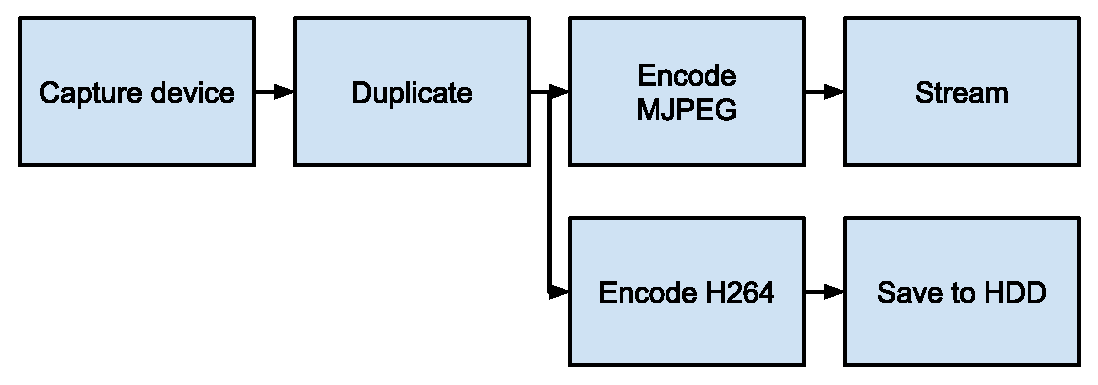
\includegraphics[width=1\textwidth]{images/yuri_example.eps}
	\caption{Libyuri -- příklad orientovaného grafu}\label{img:yuri_example}
\end{figure}

\subsection{Uzly jako fáze zpracování} \label{subsec:analyza_yuri_uzly}
Každý uzel grafu má žádný nebo více vstupů a stejně tak výstupů. Existují typy uzlů, které nemají žádný vstup ani výstup (pokud se nepodílí přímo na zpracování dat), stejně jako uzly s pevně definovaným nebo i neomezeným počtem vstupů/výstupů. Každý uzel je charakterizován svým libovolným jménem a především třídou, která reprezentuje modul, který plní funkcionalitu daného uzlu. Tedy například v ukázkovém grafu \ref{img:yuri_example} je jako první zleva uveden uzel se jménem \uv{Capture device} a může být realizován například modulem \uv{v4l2source}, který dokáže načítat video z kamery typu \textit{video4linux2}. Uzly mohou mít další množství parametrů, které jsou konkrétní každému modulu zvlášť (například zmíněný kamerový modul \textit{video4linux2} může mít další parametry typu šířka, výška, snímková frekvence a jiné).

\subsection{Hrany jako datová propojení uzlů} \label{subsec:analyza_yuri_hrany}
Orientované hrany v grafu konceptuálně představují fronty (často označované jako \textit{pipe}). Tyto fronty, realizující datová propojení uzlů, se naplňují a vyprazdňují tzv. datovými rámci (co je to datový rámec je uvedeno v sekci \ref{subsec:analyza_yuri_ramce}).

V Libyuri je aktuálně 7 různých implementací hran s různými vlastnostmi:
\begin{description}
  \item \textbf{Single\\}
Fronta o maximální délce 1 datový rámec. Má pouze 2 stavy -- prázdná a plná. Pokud dojde k zápisu nového rámce do plné fronty, starý rámec se z fronty vyhodí a zapíše se do ní nový.
  \item \textbf{Single\_blocking\\}
 Poskytuje stejné chování jako fronta \textit{Single} s tím rozdílem, že zápis do plné fronty selže (a zablokuje uzel do fronty zapisující, dokud se ve frontě neuvolní místo).
  \item \textbf{Count\_limited, Size\_limited\\}
 V těchto typech je velikost fronty omezena počtem rámců (předpona \textit{Count\_}), případně jejich celkovou velikostí (předpona \textit{size\_}).
  \item \textbf{Count\_limited\_blocking, Size\_limited\_blocking\\}
  Varianty téměř totožné s předešlými, fungující analogicky jako fronta \textit{Single\_blocking}, tedy zápis do plné fronty zablokuje zapisovací uzel do doby, než se ve frontě uvolní místo.
  \item \textbf{Unlimited\\}
Jedná se o nekonečnou frontu. Nemá žádné omezení, až na paměť počítače.
\end{description}

Uvedená množina front není omezená a je možné ji rozšiřovat.

\subsection{Datové rámce} \label{subsec:analyza_yuri_ramce}
Mezi uzly, po hranách grafu putují datové rámce (neboli \textit{frames}). Ty představují základní jednotku dat. Libyuri obsahuje hierarchii typů datových rámců z nichž nejdůležitější typy rámců jsou:
\begin{description}
  \item \textbf{Frame\\}
Obecný snímek - abstraktní třída reprezentující cokoliv, co může procházet po hranách.
  \item \textbf{RawVideoFrame\\}
Konkrétní třída reprezentující nekomprimovaný video snímek. 
  \item \textbf{CompressedVideoFrame \\}
Třída pro komprimovaný video snímek.
  \item \textbf{RawAudioFrame\\}
Třída obsahující několik vzorků nekomprimovaného audia.
\end{description}

Množina typů datových rámců se dá taktéž rozšiřovat pomocí specializace třídy \textit{Frame}.

\subsection{Vytvoření grafu} \label{subsec:analyza_yuri_vytvoreni}
Pro vytvoření grafu je možné přímo využít funkcí z API knihovny Libyuri. Pro snadnější vytváření je nicméně vhodné použít takzvaný builder. To je koncept třídy, která vytváří graf na základě nějakého vstupu. 

\subsubsection{GenericBuilder} \label{subsec:analyza_yuri_vytvoreni_generic}
Jádro obsahuje obecnou implementaci builderu pod názvem \uv{GenericBuilder}, usnadňující vytváření vlastních builderů, jako příklad je možné použít vytvořený builder \uv{SimpleBuilder} v aplikaci yuri\_simple (více o aplikaci yuri\_simple v sekci \ref{subsec:analyza_yuri_aplikace}). GenericBuilder vytváří graf specifikovaný množinou uzlů a množinou hran.

Konceptuálně představuje builder graf a zároveň je možné jej chápat jako samostatný uzel, který může být součástí většího grafu. Například předchozí ukázkový graf (\ref{img:yuri_example}) je možné rozdělit na 3 propojené podgrafy, každý vytvořený pomocí jednoho builderu, jak je patrné na grafu \ref{img:yuri_subgraph}.
\\
\begin{figure}[h]\centering
	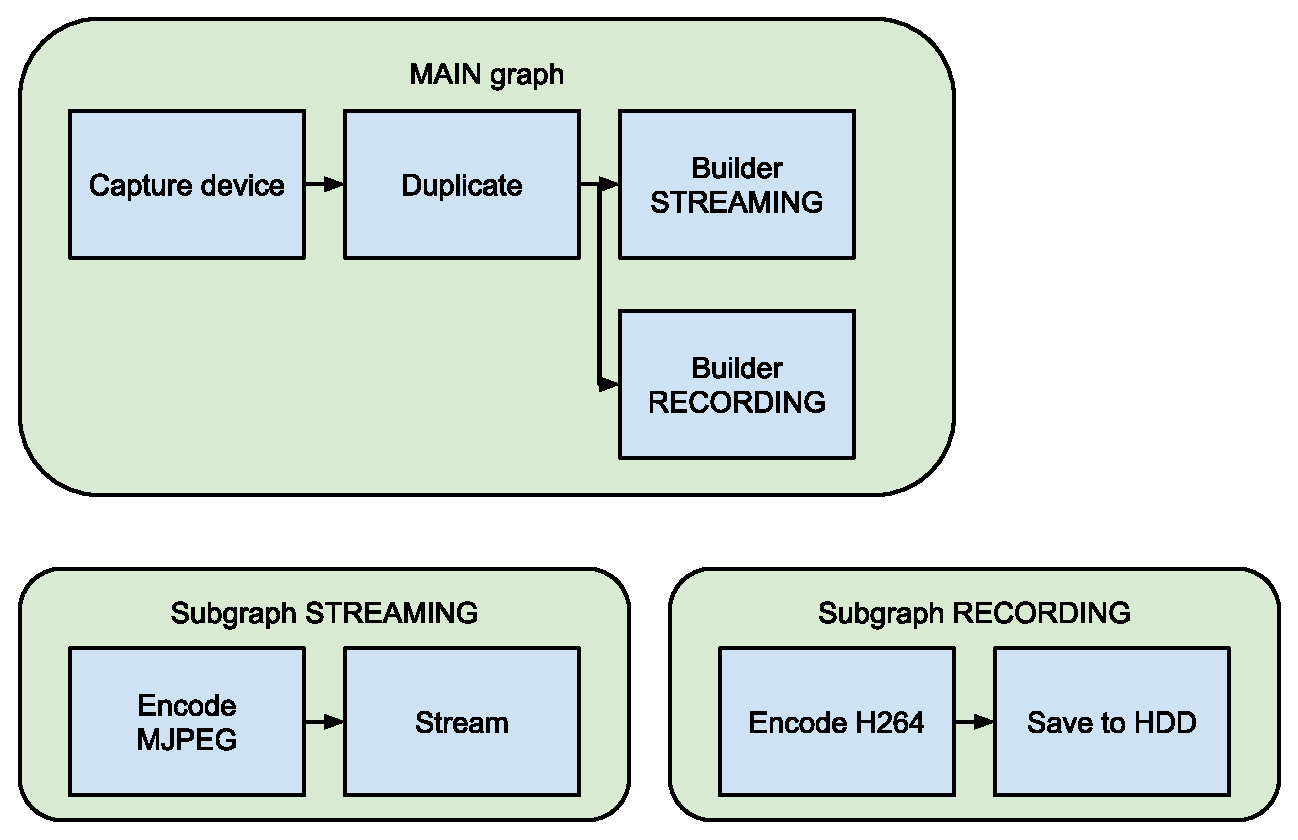
\includegraphics[width=1\textwidth]{images/yuri_subgraph.eps}
	\caption{Libyuri -- příklad propojených podgrafů pomocí builderu}\label{img:yuri_subgraph}
\end{figure}

\subsubsection{XMLBuilder} \label{subsec:analyza_yuri_vytvoreni_xml}
V jádře Libyuri je také implementace builderu \uv{XMLBuilder}, který načítá XML soubory popisující graf a datové cesty a z nich pak výsledný graf vytvoří. Použití tohoto builderu je demonstrováno dále, kde je nejprve uvedena konfigurace grafu v jazyku XML a poté vygenerovaný graf.
\\
\lstset{language=XML}
\begin{lstlisting}
<?xml version="1.0" ?>
<app name="webcam" xmlns="urn:library:yuri:xmlschema:2001"
    xmlns:xsi="http://www.w3.org/2001/XMLSchema-instance">

    <variable name="device">/dev/video0</variable>    

    <node class="v4l2source" name="webcam">
        <parameter name="path">@device</parameter>
    </node>
    <node class="sdl_window" name="sdl"/>

    <link name="yuyv_image" class="single" source="webcam:0" target="sdl:0"/>
</app>
\end{lstlisting}

V uvedené XML konfiguraci je uzel se jménem \uv{webcam} typu \uv{v4l2source}, který představuje zdroj z webkamery. Uzel nazvaný \uv{sdl} typu \uv{sdl\_window} je okno, které zobrazuje video. Mezi těmito uzly je orientovaná hrana (v Libyuri označovaná jako \textit{pipe} nebo také fronta), pojmenovaná \uv{yuyv\_image}, typu \uv{single}. Ukázková konfigurace zároveň obsahuje proměnnou (značka <variable>) obsahující systémovou cestu ke kameře. Tato proměnná je pak použita pro nastavení hodnoty parametru \uv{path} u uzlu \uv{v4l2source}. Výhody oproti přímému nastavení hodnoty (které je samozřejmě také možné) jsou dvě. Jednak je možné snadno zajistit stejnou hodnotu pro více parametrů (i v různých uzlech), ale také je možné tuto proměnnou nastavovat při spuštění yuri aplikace (více v sekci \ref{subsec:analyza_yuri_aplikace}). 

Zmíněná XML konfigurace vytvoří graf znázorněný obrázkem \ref{img:yuri_vytvoreni_xml}.
\\
\begin{figure}[h]\centering
	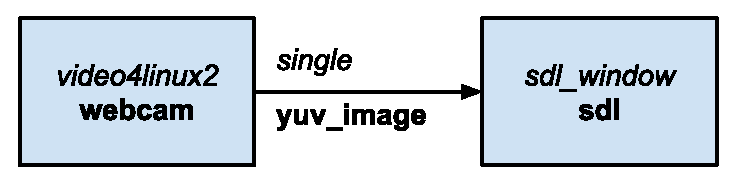
\includegraphics[width=1\textwidth]{images/yuri_xml_graph.eps}
	\caption{Libyuri -- graf vytvořený pomocí XMLBuilder}\label{img:yuri_vytvoreni_xml}
\end{figure}

XMLBuilder se chová jako každý jiný uzel a je možné ho použít v grafu. Podporuje i směrování rámců a událostí mezi vnějším a vnitřním grafem. Je tak možné napsat například složitý graf, kde vstup je reprezentován subgrafem, který je možné snadno přepnout na jiný, jak již bylo ukázáno na obrázku \ref{img:yuri_subgraph}. Stejně tak je možné takto vyměňovat libovolnou část grafu. Pokud mám například složité zapojení kamery a potřebuji výsledek někdy streamovat a někdy ukládat, tak stačí mít jednu konfiguraci pro kameru, která má finální zpracování specifikované jako subgraf. Ten pak mohu měnit (ukládání, streamování). 
Název XML souboru se pro XMLBuilder uvádí jako parametr \uv{filename}. Ten je možné samozřejmě specifikovat pomocí proměnné, která se dá při spuštění nastavit na jinou hodnotu. 
\\ \\
Kompletní popis builderu XMLBuilder je v souboru \textit{doc/XMLBUILDER.txt} v distribuci Libyuri.

\subsection{Události} \label{subsec:analyza_yuri_udalosti}
Propojení uzlů v grafu pomocí hran definuje datové cesty pro audio/video data. Kromě toho je ale také možné mezi uzly posílat události (tzv. \textit{events}). Každá událost má svůj typ a hodnotu (například \textit{bool} a \textit{false}, nebo \textit{double} a \textit{3.14}). V Libyuri existují následující typy událostí:

\begin{labeling}{Dictionary12}
\item [\textbf{Bool}] Hodnota \textit{true} nebo \textit{false}.
\item [\textbf{Int}] Celočíselná hodnota, omezená na 64 bitů. Volitelně může mít i specifikovaný rozsah do kterého patří.
\item [\textbf{Double}] Hodnota s plovoucí desetinnou čárkou, omezená na 128 bitů. Volitelně může mít specifikovaný rozsah.
\item [\textbf{String}] Textová hodnota.
\item [\textbf{Time}] Časová známka.
\item [\textbf{Vector}] Uspořádaná množina událostí (heterogenních typů)
\item [\textbf{Dictionary}] Slovník mapující hodnoty typu \textit{String} na události (heterogenních typů)
\item [\textbf{BANG}] Specialní typ, kerý nemá hodnotu.
\end{labeling}

Uzel, který implementuje koncept \uv{BasicEventProducer} může generovat (\textit{emit\_event}) dvojice jméno a událost. Uzel sám neřeší kam se událost posílá. Oproti tomu uzel, který implementuje koncept \uv{BasicEventConsumer} umí dvojice jméno a událost přijímat. Jaká událost se kam posílá se specifikuje zvlášť v konfiguraci.\\

Dále je uveden jednoduchý příklad XML kódu demonstrující události.
\\
\lstset{language=XML}
\begin{lstlisting}
<event>
  route(dump:sequence) -> info:progress;
</event>
\end{lstlisting}

Pokud se zanese tento příklad do existující XML konfigurace grafu, tak ve chvíli, kdy uzel pojmenovaný \uv{dump} vygeneruje událost s názvem \uv{sequence}, tak se ta událost pošle do uzlu \uv{info} pod názvem \uv{progress}.

Specifikace směrování podporuje i funkcionální jazyk pro modifikaci událostí nebo kombinující více událostí dohromady. Je tak možné vytvářet i složitější konstrukce jak v příkladu uvedeném dále.
\\
\lstset{language=XML}
\begin{lstlisting}
<event>
  route(gt(dump:sequence, var:max_frames)) -> generate:stop;
</event>
\end{lstlisting}

Tento trochu komplexnější příklad vezme hodnotu události \uv{sequence} z uzlu \uv{dump}, porovná ji (funkce \textit{gt}) s hodnotou události \uv{max\_frames} z uzlu \uv{var} a výsledek (hodnota \textit{true} nebo \textit{false}) se pošle na uzel \uv{generate} jako událost s názvem \uv{stop}.
\\ \\
Detailnější popis událostí je v souboru \textit{doc/EVENTS.txt} v distribuci Libyuri.
	
\subsection{Moduly} \label{subsec:analyza_yuri_moduly}
Jak již bylo zmíněno v sekci o uzlech grafu zpracování audia/videa (\ref{subsec:analyza_yuri_uzly}), každý uzel je charakterizován třídou, která reprezentuje modul plnící funkcionalitu daného uzlu. Jako modul je označována dynamická knihovna (například \textit{yuri2.8\_module\_v4l2\_source.so}), která může obsahovat dodatečné funkce pro Libyuri. Typicky takový modul obsahuje jeden nebo více uzlů do grafu, může ale obsahovat i jiné funkce (například modul \textit{yuri2.8\_module\_yuri\_udp.so} obsahuje implementaci konceptu \textit{DatagramSocket} pomocí UDP soketu). 

Moduly se kompilují samostatně, mohou být umístěny i mimo distribuci Libyuri. Pro kompilaci modulu je nutné pouze dostupné API Libyuri a knihovna \textit{yuri2.8\_core}, se kterou se linkují. Aplikace, které využívají Libyuri (vizte \ref{subsec:analyza_yuri_aplikace}) se linkují pouze s jádrem knihovny. Po spuštění aplikace, jádro (pomocí builderu) vyhledá moduly v adresářích napevno uvedených v kódu a případně dalších, specifikovaných uživatelem a načte je.

\subsection{Aplikace používájící libyuri} \label{subsec:analyza_yuri_aplikace}
Jako součást knihovny Libyuri je distribuováno několik aplikací, které tuto knihovnu používají. Dále jsou uvedeny 3 nejdůležitější pro implementaci řešení této práce.\\

\begin{description}
  \item \textbf{Yuri\_simple\\}
  Program pro vytváření grafů bez konfiguračního XML souboru. Všechny potřebné informace k vytvoření grafu se předají argumenty při spuštění programu. Například následující příkaz spustí stejnou konfiguraci jako ukázkový příklad grafu ze sekce XMLBuilder (\ref{subsec:analyza_yuri_vytvoreni_xml}).\\
  
\lstset{language=bash,morekeywords={yuri_simple,v4l2source, path, dev, video0, sdl_window},keywordstyle=\color{black}}
\begin{lstlisting}
./yuri_simple v4l2source[path=/dev/video0] sdl_window
\end{lstlisting}

  \item \textbf{Yuri\_test\_module\\}
  Aplikace testující validitu modulů. Následující příkaz otestuje, jestli je modul \textit{yuri2.8\_module\_null.so} validní.
\lstset{language=bash,alsoletter={.},morekeywords={yuri_test_module, yuri2.8_module_null.so},keywordstyle=\color{black}}
\begin{lstlisting}
./yuri_test_module yuri2.8_module_null.so
\end{lstlisting}

  \item \textbf{Yuri2\\}
Tento program načítá konfigurační XML soubor (vizte popis XMLBuilderu \ref{subsec:analyza_yuri_vytvoreni_xml}) a spouští aplikaci v něm popsanou. Následuje nejjednodušší příklad spuštění tohoto programu.\\

\lstset{language=bash,morekeywords={yuri2,\$, config, xml},keywordstyle=\color{black}}
\begin{lstlisting}
./yuri2 config.xml
\end{lstlisting}

Pokud jsou v konfiguračním souboru uvedeny proměnné (značky <variable>, stejné, jako v příkladu \ref{subsec:analyza_yuri_vytvoreni_xml}), je možné jim nastavit hodnotu na příkazové řádce tak, jako v následujícím příkladu, kde se nastaví proměnná \uv{device}.\\

\lstset{language=bash,morekeywords={yuri2,\$, config, xml, device, video0, dev},keywordstyle=\color{black}}
\begin{lstlisting}
./yuri2 config.xml device=/dev/video0
\end{lstlisting}

Aplikace \textit{yuri2} má množství dalších parametrů, pro jejich seznam stačí spustit aplikaci bez parametrů a zobrazí se základní nápověda. Mezi důležité parametry patří:

\begin{description}
	\item[-a] Vypíše informace o zadaném konfiguračním souboru.
	\item[-v] Detailnější výpisy, \textbf{-q} je méně detailní výpis.
	\item[-L class] Vypíše informace o třídě \uv{class}.
	\item[-l {[what]}] Bez uvedeného argumentu \textit{what} (nebo pokud je tento argument \uv{classes}) vypíše seznam registrovaných tříd. Pokud je argument \uv{pipes}, tak vypíše seznam tříd pro \textit{pipes} neboli fronty.
	\item[-C format1:format2] Vypíše, pokud je možná automatická konverze z formátu \uv{format1} do \uv{format2} a vypíše, jaké uzly by tuto konverzi realizovaly.
\end{description}

\end{description}


\chapter{Návrh} \label{chap:navrh}
Návrh nejprve rozebere architekturu systému a pak ve dvou podkapitolách proběhne návrh frontendové (prezentační vrstva aplikace, která systému předkládá vstupy od uživatele a zároveň uživateli zobrazuje výstupy) a backendové (kde je uvedeno, jaká je struktura té části aplikace, která je uživateli odstíněna, ale která také zajišťuje většinu funkcionalit) části řešení.

\section{Architektura systému} \label{sec:navrh_architektura}
Řešení bude navrženo, jako typická třívrstvá architektura skládající se z prezentační aplikační a datové vrstvy. Prezentační vrstva zahrnuje frontend \ref{sec:navrh_frontend} a jeho zprostředkování pomocí webového serveru. Aplikační vrstva pojímá aplikační server (server v laboratoři CHUL) včetně nahrávacích zařízení a komunikace mezi nimi pomocí knihovny Libyuri. Datová vrstva se pak skládá z PostgreSQL databáze a úložiště veškerých nahrávek.

\subsubsection{Diagram nasazení} \label{subsubsec:navrh_architektura_nasazeni}
Schéma na obrázku \ref{img:navrh_architektura_nasazeni} uvedeném dále představuje přibližný model nasazení v provozu. Tento model se skládá ze čtyř hlavních částí (zařízení), z nichž první představuje klienta a jeho webový prohlížeč. Ten komunikuje
s aplikací Nginx, která představuje webový server. Samotná komunikace mezi klientem a webovým serverem probíhá pomocí protokolů HTTPS a SFTP pro procházení webové aplikace a případný download videí. Aplikace Nginx hostuje samotnou webovou aplikaci, jejíž podstatná část je tvořena PHP frameworkem Nette a dále Javascriptovou knihovnu Video.js (\ref{subsubsec:analyza_reseni_videojs}), která je odpovědná za práci s videem na webu. Další částí diagramu je CHUL server, neboli server, nacházející se v CHUL laboratoři, na kterým běží instance knihovny Libyuri (\ref{subsubsec:analyza_reseni_yuri}).  Komunikace mezi Libyuri a webovou Nette aplikací je zajištěno technologií websocketů, pomocí kterých se například z webové aplikace pošle příkaz na spuštění nahrávání z různých zařízení v laboratoři. K operačnímu systému CHUL serveru je pomocí techologie SSHFS připojen souborový systém dalšího a posledního zařízení v diagramu -- databázového a multimediálního serveru (Dále jen \uv{DM server}). Tento DM server obsahuje zmíněnou databázi PostgreSQL a také úložiště pro nahrané záznamy. Databázový systém PostgreSQL na DM serveru obsahuje především data potřebné webovou aplikací (jako jsou data o uživatelích, experimentech, scénářích a jiné) a tudíž je se samotnou webovou aplikací spojena komunikačním protokolem TCP/IP. 
\\
\begin{figure}[h]\centering
	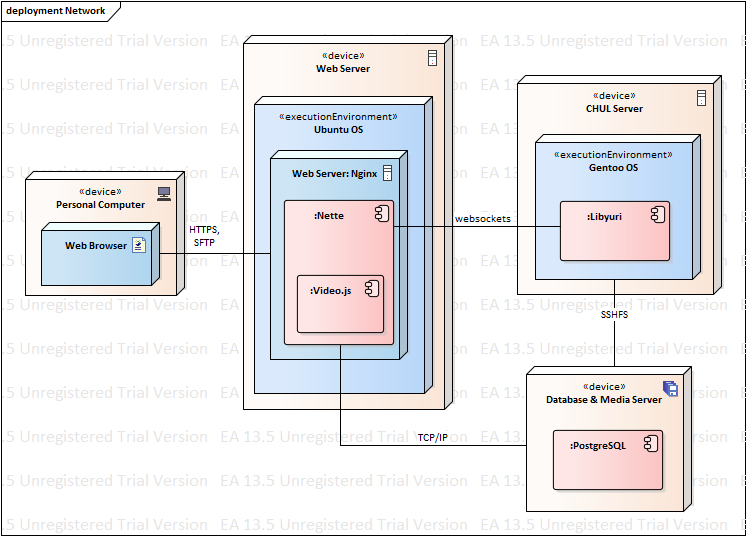
\includegraphics[width=1\textwidth]{images/nasazeni.png}
	\caption{Diagram nasazení}\label{img:navrh_architektura_nasazeni}
\end{figure}


\section{Frontend} \label{sec:navrh_frontend}

\subsection{Uživatelské rozhraní}
Tato sekce se věnuje návrhu a tvrobě UI (User Interface) frontendové části řešení. Se zužitkováním znalostí z \cite{nur} je využito ověřených postupů a je kladen důraz na principy dobrého UI jako jsou jednolitost, předpovídatelnost, zobrazování pouze užitečných informací, tolerance chyb a další. 

Návrh uživatelského rozhraní rozdělen na několik fází. Prvním krokem je seznam požadavků a vlastností kladených na uživatelské rozhraní. Tyto požadavky jsou již stanoveny v analýze (\ref{sec:analyza_pozadavky}). Zmíněné požadavky a vlastnosti jsou poté, po poradě s vedoucím práce, transformovaný do takzvaného task listu, jehož finální podoba obsahuje uspořádaný seznam základních funkcionalit UI z uživatelova pohledu. Dalším krokem, dle uznávaných postupů, by byl výběr cílové skupiny uživatelů tohoto systému a uživatelský výzkum. Cílová skupina uživatelů je však již známa díky již existující webové aplikaci, jejíž koncepty budou pro první prototypy UI této práce postačující. Uživatelské testování je tak tedy provedeno až na prvních prototypech řešení a je částečně zmíněno v kapitole o testování (\ref{subsec:testovani_akceptacni_utest}). Pro zvýraznění struktury závislostí mezi funkcionalitami task listu bude vytvořen tzv. task graf (nebo také task model), který znázorní vztahy mezi jednotlivými funkcionalitami. Nakonec se vytvoří hi-fi prototyp, který bude reprezentovat grafickou a interaktivní podobu uživatelského rozhraní.

\subsubsection{Task List} \label{subsubsec:navrh_frontend_ui_tasklist}
Zde je uveden seznam většiny úkolů, které by mělo uživatelské rozhraní splňovat, jakožto požadavky uživatelů. Pokud se ve vytvořeném seznamu nedopatřením neobjevily věci, které tam být mají, tak by se měly ukázat při testování použitelnosti uživatelského rozhraní.

\begin{itemize}
 \item Zobrazení zařízení schopných nahrávání.
 \item Označení skupiny zařízení pro nahrávání
 \item Volba streamu do systému SAGE
 \item Spuštění nahrávání (streamování)
 \item Přidávání komentáře ke streamu
 \item Zastavení nahrávání (streamování)
 \item Zobrazení streamovaného obrazu
 \item Spuštění editoru/přehrávače nahrávek
 \item Zobrazení existujících nahrávek
 \item Přehrání vybrané nahrávky
 \item Změna hlasitosti přehrávání
 \item Změna rychlosti přehrávání
 \item Změna rozlišení přehrávání
 \item Spuštění přehrávání na celou obrazovku
 \item Zobrazení komentářů videa
 \item Sloučení nahrávek paralelně do mřížky
 \item Volba časového ořezu videa 
 \item Rotace obrazu videa
 \item Změna kontrastu obrazu videa
 \item Volba rozlišení pro export
 \item Volba formátu pro export
 \item Volba uploadu záznamu na server YouTube
 \item Zobrazení editovatelných meta-informací
 \item Návrat z editoru do streamování
 \item Zobrazení volného místa v úložišti
\end{itemize}

Dále je nutné tento neorganizovaný seznam funkcionalit seskupit tak, aby to co nejlépe pomohlo s návrhem UI. Tasky se seskupují například podle toho, zda-li se jedná o vstup od uživatele, oznámení chyb, jak velkou část obrazovky zaujímají a podobně. Některé položky v seznamu mohou být syntaxí skryté duplicity jiných. Zároveň je žádoucí seřadit položky dle jejich důležitosti (například chybové hlášky mají vysokou prioritu).

\begin{itemize}
 \item Nastavení streamování
   \begin{itemize}
	 \item Zobrazení zařízení schopných nahrávání.
	 \item Označení skupiny zařízení pro nahrávání
	 \item Volba streamu do systému SAGE
	 \item Sloučení streamů paralelně do mřížky
	 \item Rotace obrazu streamu
	 \item Spuštění nahrávání (streamování)
   \end{itemize}
 \item Zobrazení streamovaného obrazu
   \begin{itemize}
	 \item Zastavení nahrávání (streamování)
 	 \item Přidávání komentáře ke streamu
   \end{itemize}
 \item Spuštění editoru/přehrávače nahrávek
 \item Zobrazení existujících nahrávek
 \item Přehrání vybrané nahrávky
   \begin{itemize}
 	 \item Změna hlasitosti přehrávání
	 \item Změna rychlosti přehrávání
	 \item Změna rozlišení přehrávání
 	 \item Spuštění přehrávání na celou obrazovku
 	 \item Zobrazení komentářů videa
   \end{itemize}
 \item Úprava videa pro export
   \begin{itemize}
	 \item Volba časového ořezu videa 
     \item Změna kontrastu obrazu videa
  	 \item Volba rozlišení pro export
  	 \item Volba formátu pro export
	 \item Zobrazení editovatelných meta-informací
	 \item Volba uploadu záznamu na server YouTube
   \end{itemize}
 \item Zobrazení volného místa v úložišti
 \item Návrat z editoru do nastavení streamování
\end{itemize}

\subsubsection{Task Graf} \label{subsubsec:navrh_frontend_ui_taskgraf}
Zde jsou zobrazeny task grafy vytvořené ze zmíněného task listu. Byly vytvořeny grafy dva, přičemž jeden se týká oblasti nastavování streamování a náhledu probíhajícího streamování (obrázek \ref{img:navrh_frontend_ui_taskgraf_1}) a druhý se týká webového videopřehrávače a editoru (obrázek \ref{img:navrh_frontend_ui_taskgraf_2}). V grafech jsou znázorněny závislosti mezi uživatelskými akcemi reprezentované řádkami v task listu. Je v nich náčrt rozvržení webových stránek (modrý obdélník) a jednotlivých akcí (žlutý obdélník) na každé z těchto stran.
\\
\begin{figure}[h]\centering
	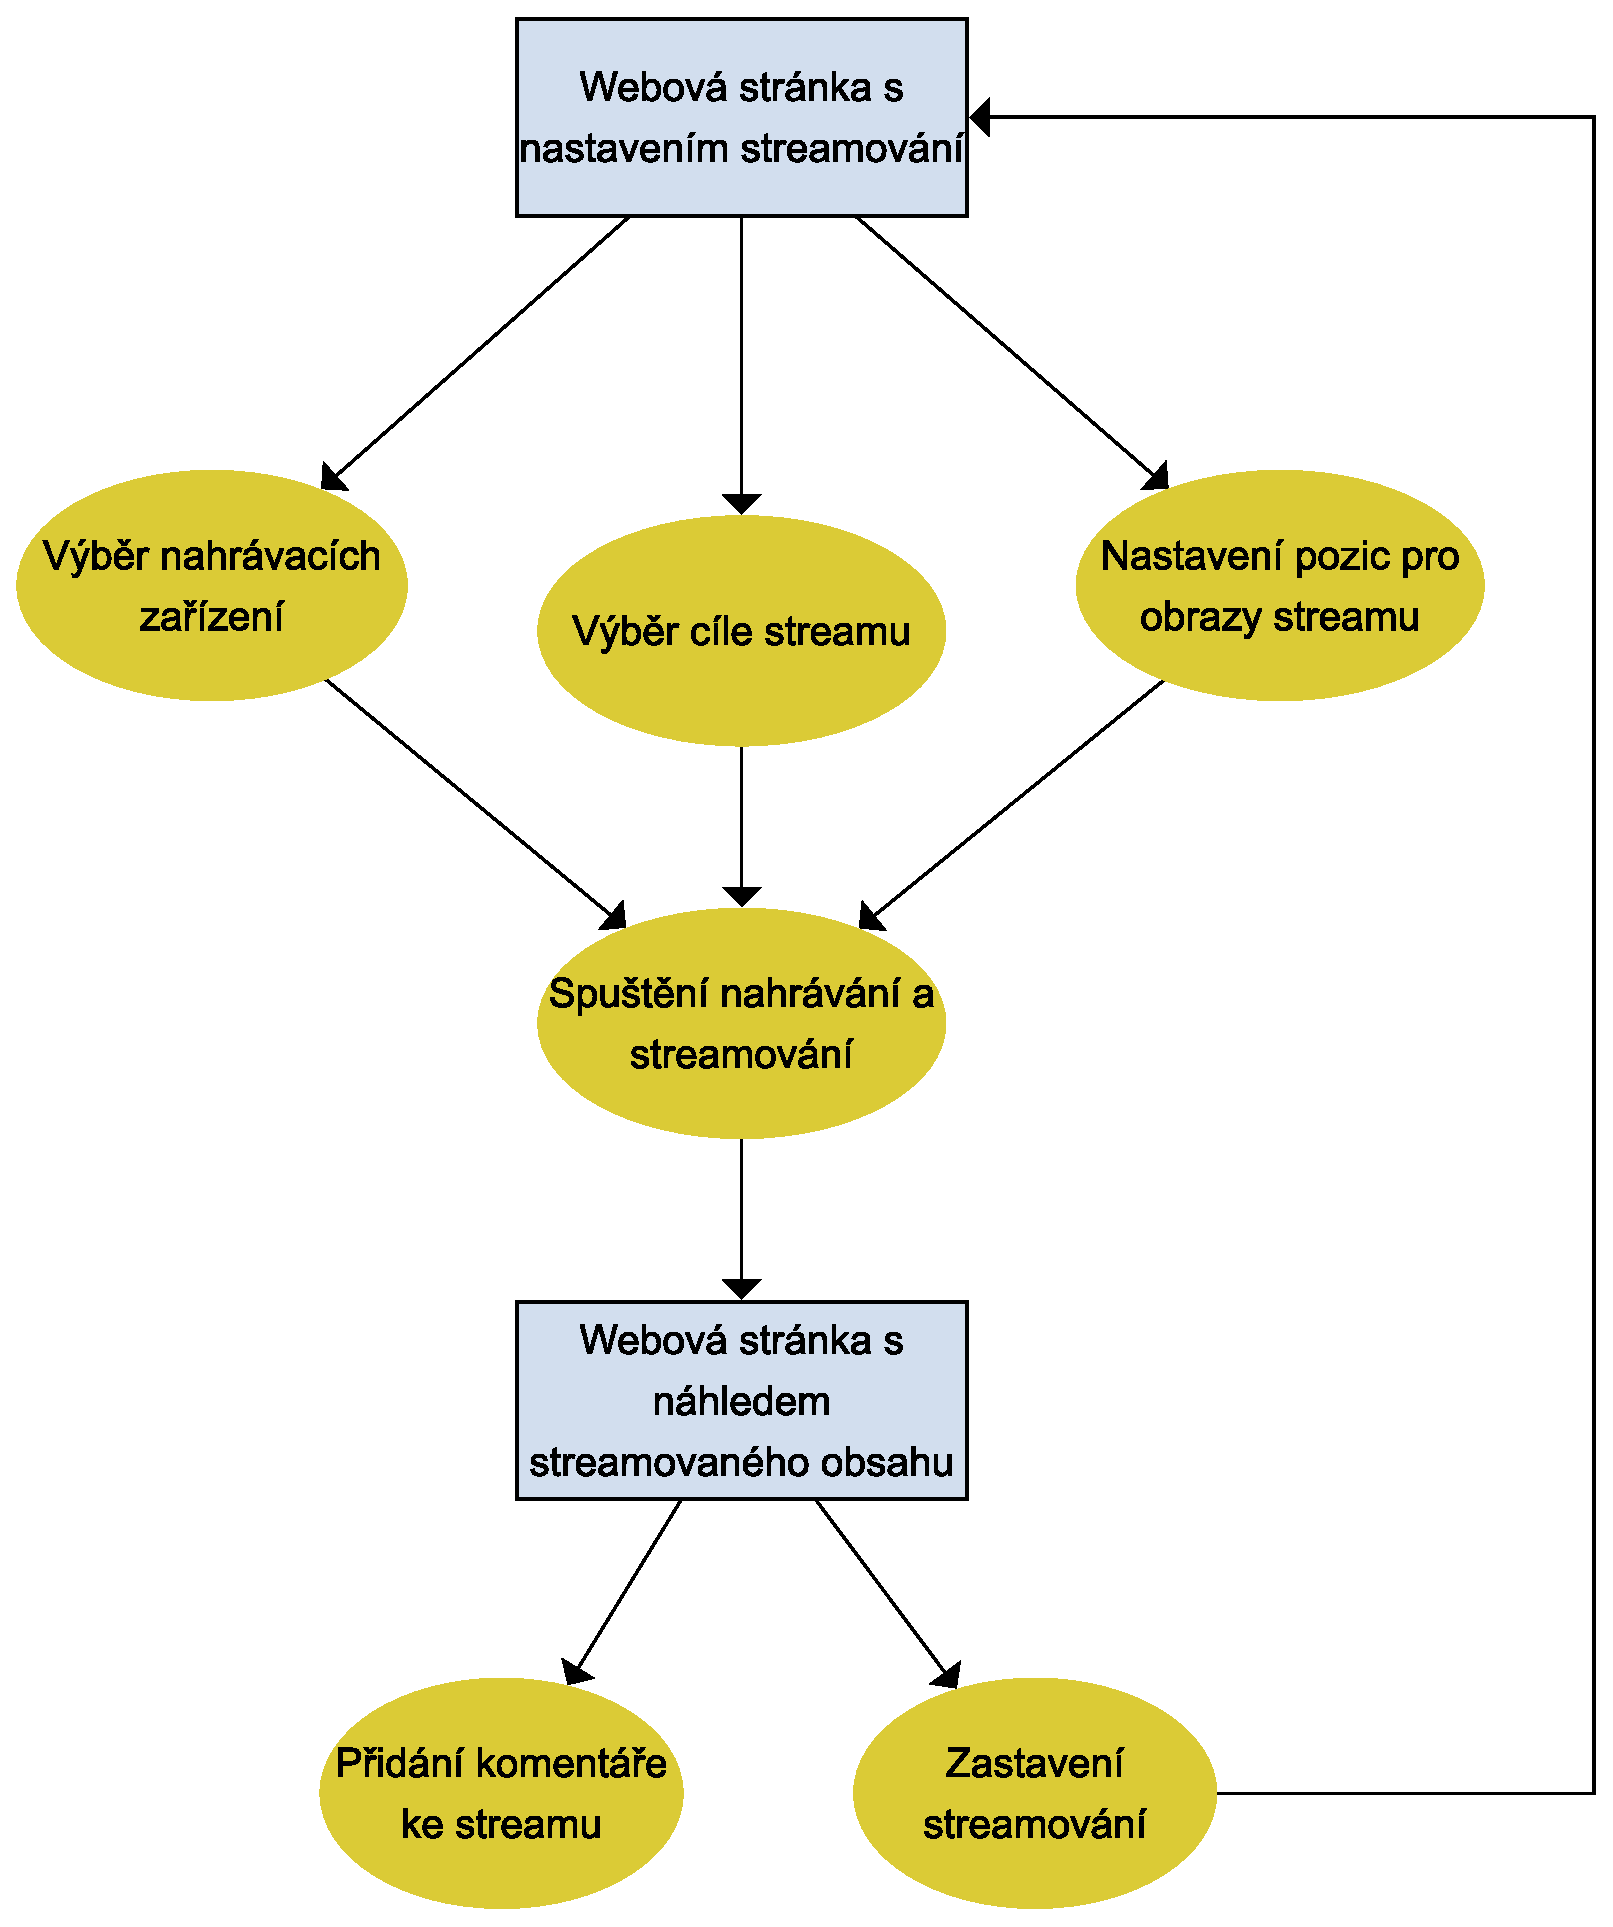
\includegraphics[width=0.7\textwidth]{images/ui_task_flow_1.eps}
	\caption{Task graf pro nastavení a náhled streamování}\label{img:navrh_frontend_ui_taskgraf_2}
\end{figure}
\\
\begin{figure}[h]\centering
	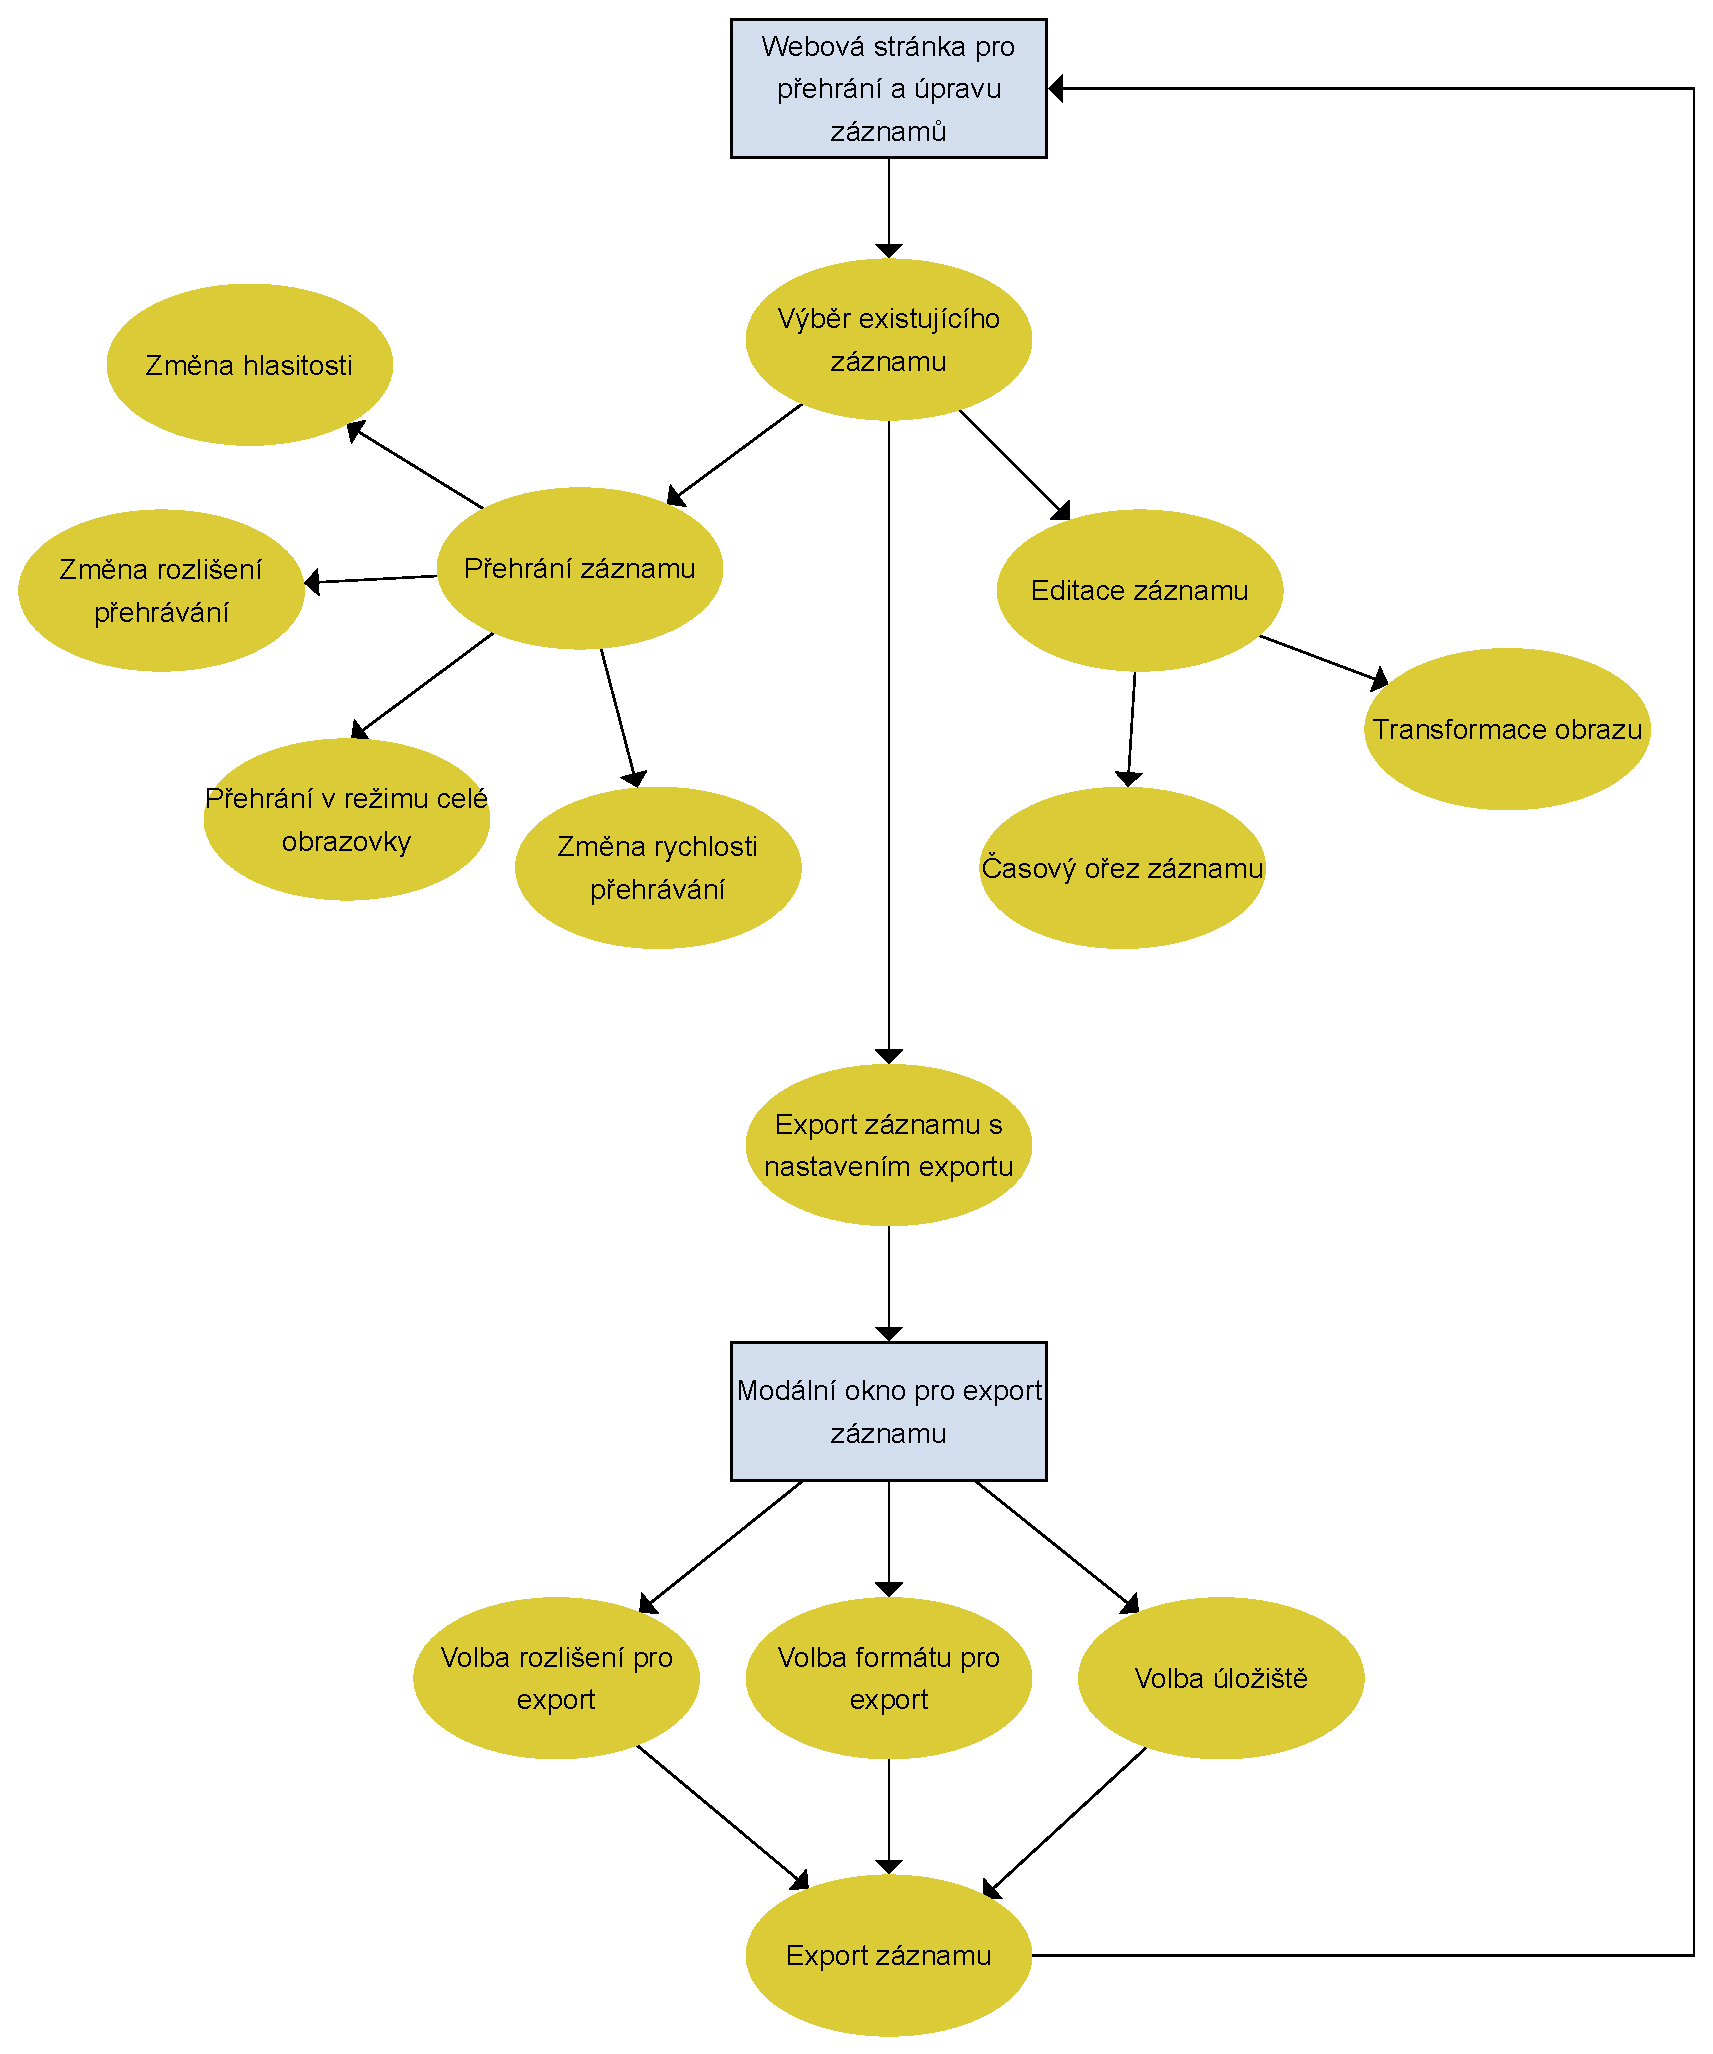
\includegraphics[width=1\textwidth]{images/ui_task_flow_2.eps}
	\caption{Task graf pro video přehrávač a editor}\label{img:navrh_frontend_ui_taskgraf_1}
\end{figure}

\subsubsection{Prototypování} \label{subsubsec:navrh_frontend_ui_proto}
Z již uspořádaného task listu a z něj vytvořených task grafů je patrné, že pro realizaci UI jsou potřeba tři webové stránky (jedna pro přehrávání a úpravu záznamů, další pro nastavení a spuštění nahrávání/streamování a třetí pro sledování průběhu nahrávání/streamování) a jedno modální okno pro nastavení exportu videí ve video editoru. Byly tedy vytvořeny prototypy stránek jako wireframe. Nejprve se prototypy načrtly na papír ke zjištění základních nedostatků a později se z těchto náčrtů vytvořil interaktivní wireframe. Při tvorbě wireframu se dá postupovat metodou \uv{od shora} (nejprve návrh hlavního rozvržení stránky a poté zaměření na jednotlivé komponenty) či \uv{od zdola} (opak k předchozí metodě). Zde se však postupovalo kombinovaně, tedy nejprve se promyslely komponenty a s vědomím potřebného místa pro ně se navrhovalo rozvržení stránky. 

	Prototyp UI je zde zobrazen jako screenshoty stránek interaktivních wireframu a to čtyřmi obrázky. Obrázek \ref{img:navrh_frontend_ui_wf_config} představuje webovou stránku s nastavením nahrávání a streamování. V sekci o nastavení streamování v task listu (vizte \ref{subsubsec:navrh_frontend_ui_tasklist}) se první dva body týkají zobrazení zařízení schopných nahrávání a jejich následného výběru. Pro tyto funkcionality se alokovala horní část stránky, která obsahuje horizontální seznam zařízení spolu s jejich náhledy. Dále byla zabrána střední část webové stránky, tedy hlavní část obsahu, ve které si bude uživatel moci stanovit pozice jednotlivých kamer. Dále je do pravé spodní části obrazovky přidáno tlačítko pro spuštění nahrávání a streamování. V poslední řadě jsou nad tímto tlačítkem oblast věnována nastavení cíle streamu a podobně.

Na obrázku \ref{img:navrh_frontend_ui_wf_preview} je stránka wireframu pro sledování průběhu streamování. V task listu jsou v sekci o náhledu streamování pouze tři hlavní tasky -- zobrazení streamovaného obsahu, možnost přidání komentáře ke streamu a zastavení streamování. Zastavení streamování je tlačítko podobné funkcionality jako spuštění streamování v obrazovce na obrázku  \ref{img:navrh_frontend_ui_wf_config} a tak je žádoucí pro něj alokovat prostor na stejném místě v obrazovce. Stejně tak zobrazení streamovaného obsahu, které bude mít stejný tvar a obdobnou velikost jako prostor s vybranými kamerami z obrázku\ref{img:navrh_frontend_ui_wf_config}, zaujme stejné místo v prostoru obrazovky. Zbylé místo v pravé části nad tlačítkem pro zastavení streamování pak zabere funkcionalita pro přidání komentářů a případně zobrazení nedávno přidaných. 

Třetí a nejzajímavější obrazovka z wireframu v řadě, na obrázku \ref{img:navrh_frontend_ui_wf_editor}, se týká přehrávače a editoru videí. Této obrazovky se týka ta část task listu od bodu \uv{Spuštění editoru/přehrávače nahrávek} až do konce, přičemž pro část s úpravou videa pro export je věnováno modální okno vyjádřené obrázkem \ref{img:navrh_frontend_ui_wf_export}. Obrazovka pro videopřehrávač a editor nejprve v levé horní části obsahuje název projektu a ikonku pro export, která zobrazí zmíněné a dále popsané modální okno. Pod těmito prvky je rozvedený seznam různých nahrávek daného projektu. V pravé části obrazovky je pak samotný videopřehrávač, který přehrává media sestavená ve spodní části obrazovky na časové ose. Tato časová osa je rozdělena na tři části, jedna obsahuje videa, další audio stopy a poslední titulky, které byly generovány jako komentáře během streamování. Časová osa zobrazuje upravovaná media rozprostřená v čase zleva doprava. Zmíněné titulky/komentáře jsou pak ještě zobrazovány pod videopřehrávačem během přehrávání. Poslední a zároveň jedna z nejdůležitějších částí obrazovky je oblast mezi časovou osou a horní částí webové stránky. Nachází se zde pásová oblast, která obsahuje většinu kontrolních prvků pro práci s videem. Zleva jsou zde ikony pro střih videa, kopírování a mazání elementů časové osy, práci se zvukem přehrávaného videa, přidání médií na časovou osu, v další části pak spouštění, pozastavování a přetáčení přehrávaného obsahu a nakonec ikona pro nastavení obsahující například změnu rozlišení přehrávání či přepnutí do celoobrazovkového režimu.

	Po kliknutí na ikonu exportu vedle názvu projektu, na stránce s videopřehrávačem a editorem, se otevře modální okno s nastavením pro export. Toto okno je sestaveno na obrázku poslední obrazovky wireframu (\ref{img:navrh_frontend_ui_wf_export}). Modální okno pro export pak pokrývá poslední část task listu od položky \uv{Úprava videa pro export} do konce. V oknu je nejprve uvedeno jméno projektu, který se bude exportovat a dále pak základní množina nastavení. Mezi tyto nastavení patří rozlišení obrazu videa, snímková frekvence a formát videa. Dále je zde možnost volby úložiště spolu se zobrazeným dostupným volným místem. Krom tlačítka pro export, které všechna nastavení aplikuje a video vyexportuje, je zde ještě možnost nahrát projekt na server YouTube pod zadaným jménem, do již předem stanoveného kanálu pro CHUL. Konečně je zde také políčko pro mailovou adresu, na kterou může přijít notifikace při dokončení exportu.
\\
\begin{figure}[h]\centering
	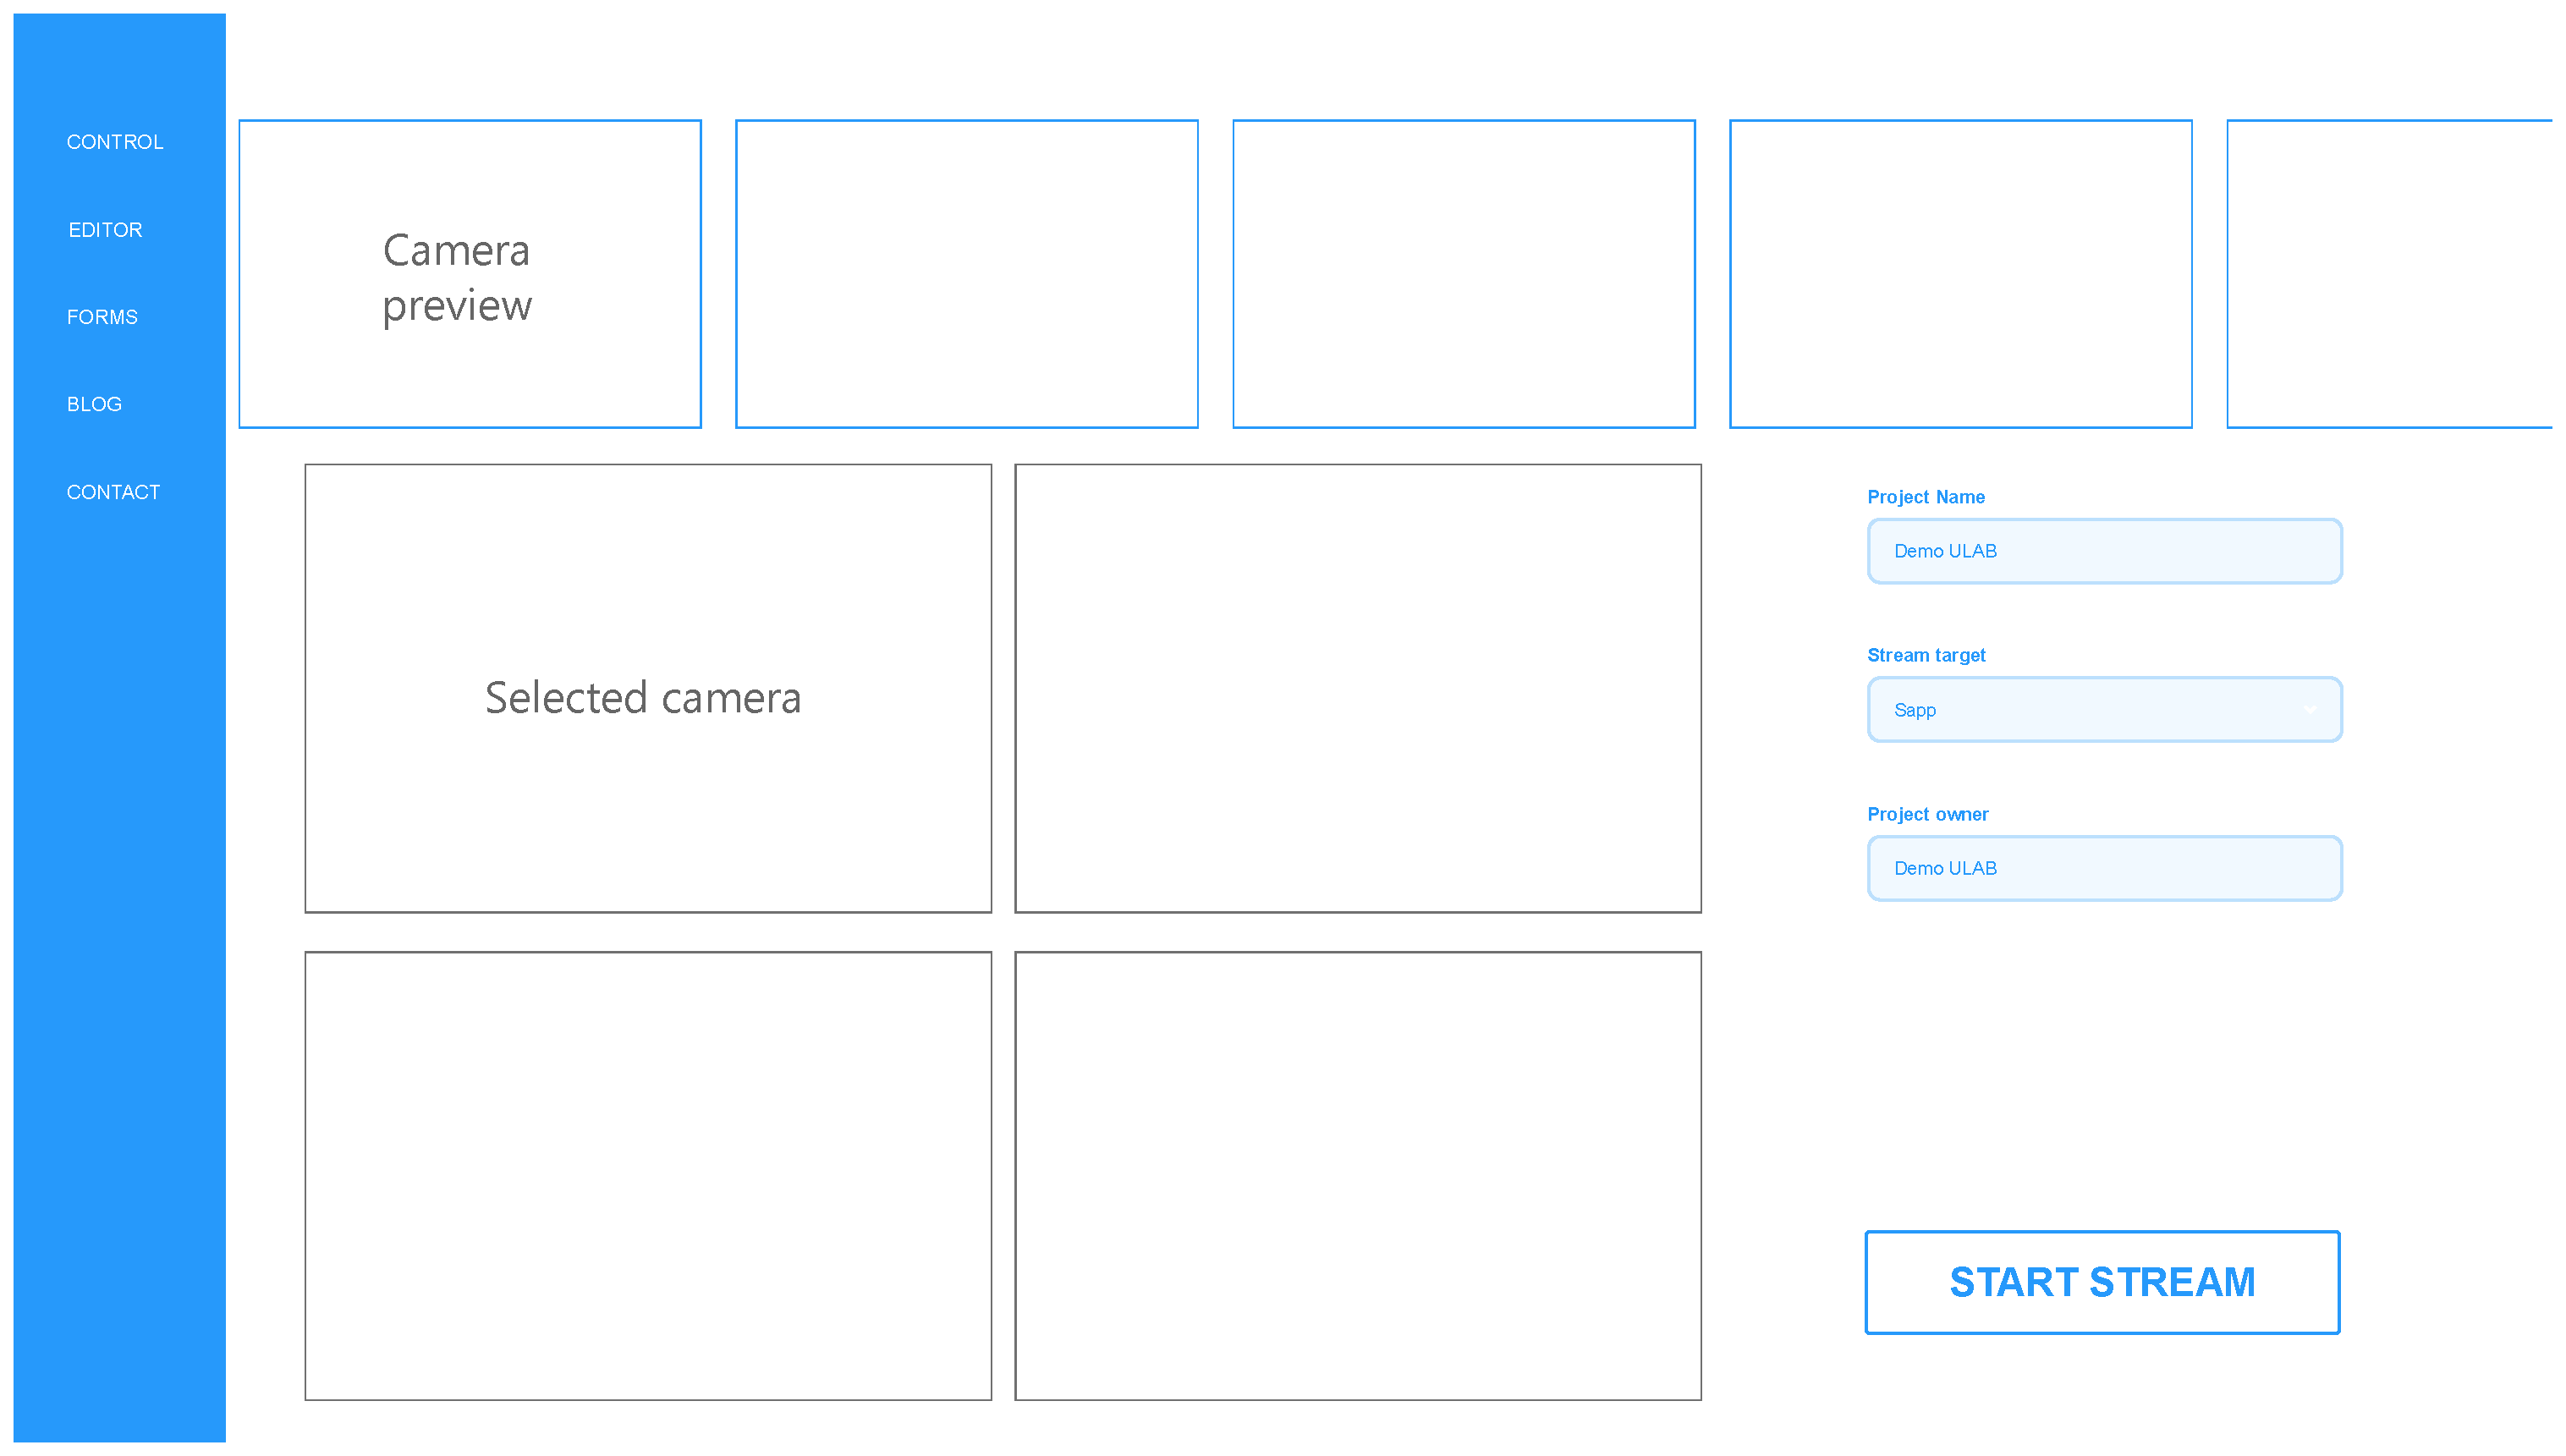
\includegraphics[width=1\textwidth]{images/ui_wf_ulab-config.eps}
	\caption{Wireframe pro nastavení streamování}\label{img:navrh_frontend_ui_wf_config}
\end{figure}
\\
\begin{figure}[h]\centering
	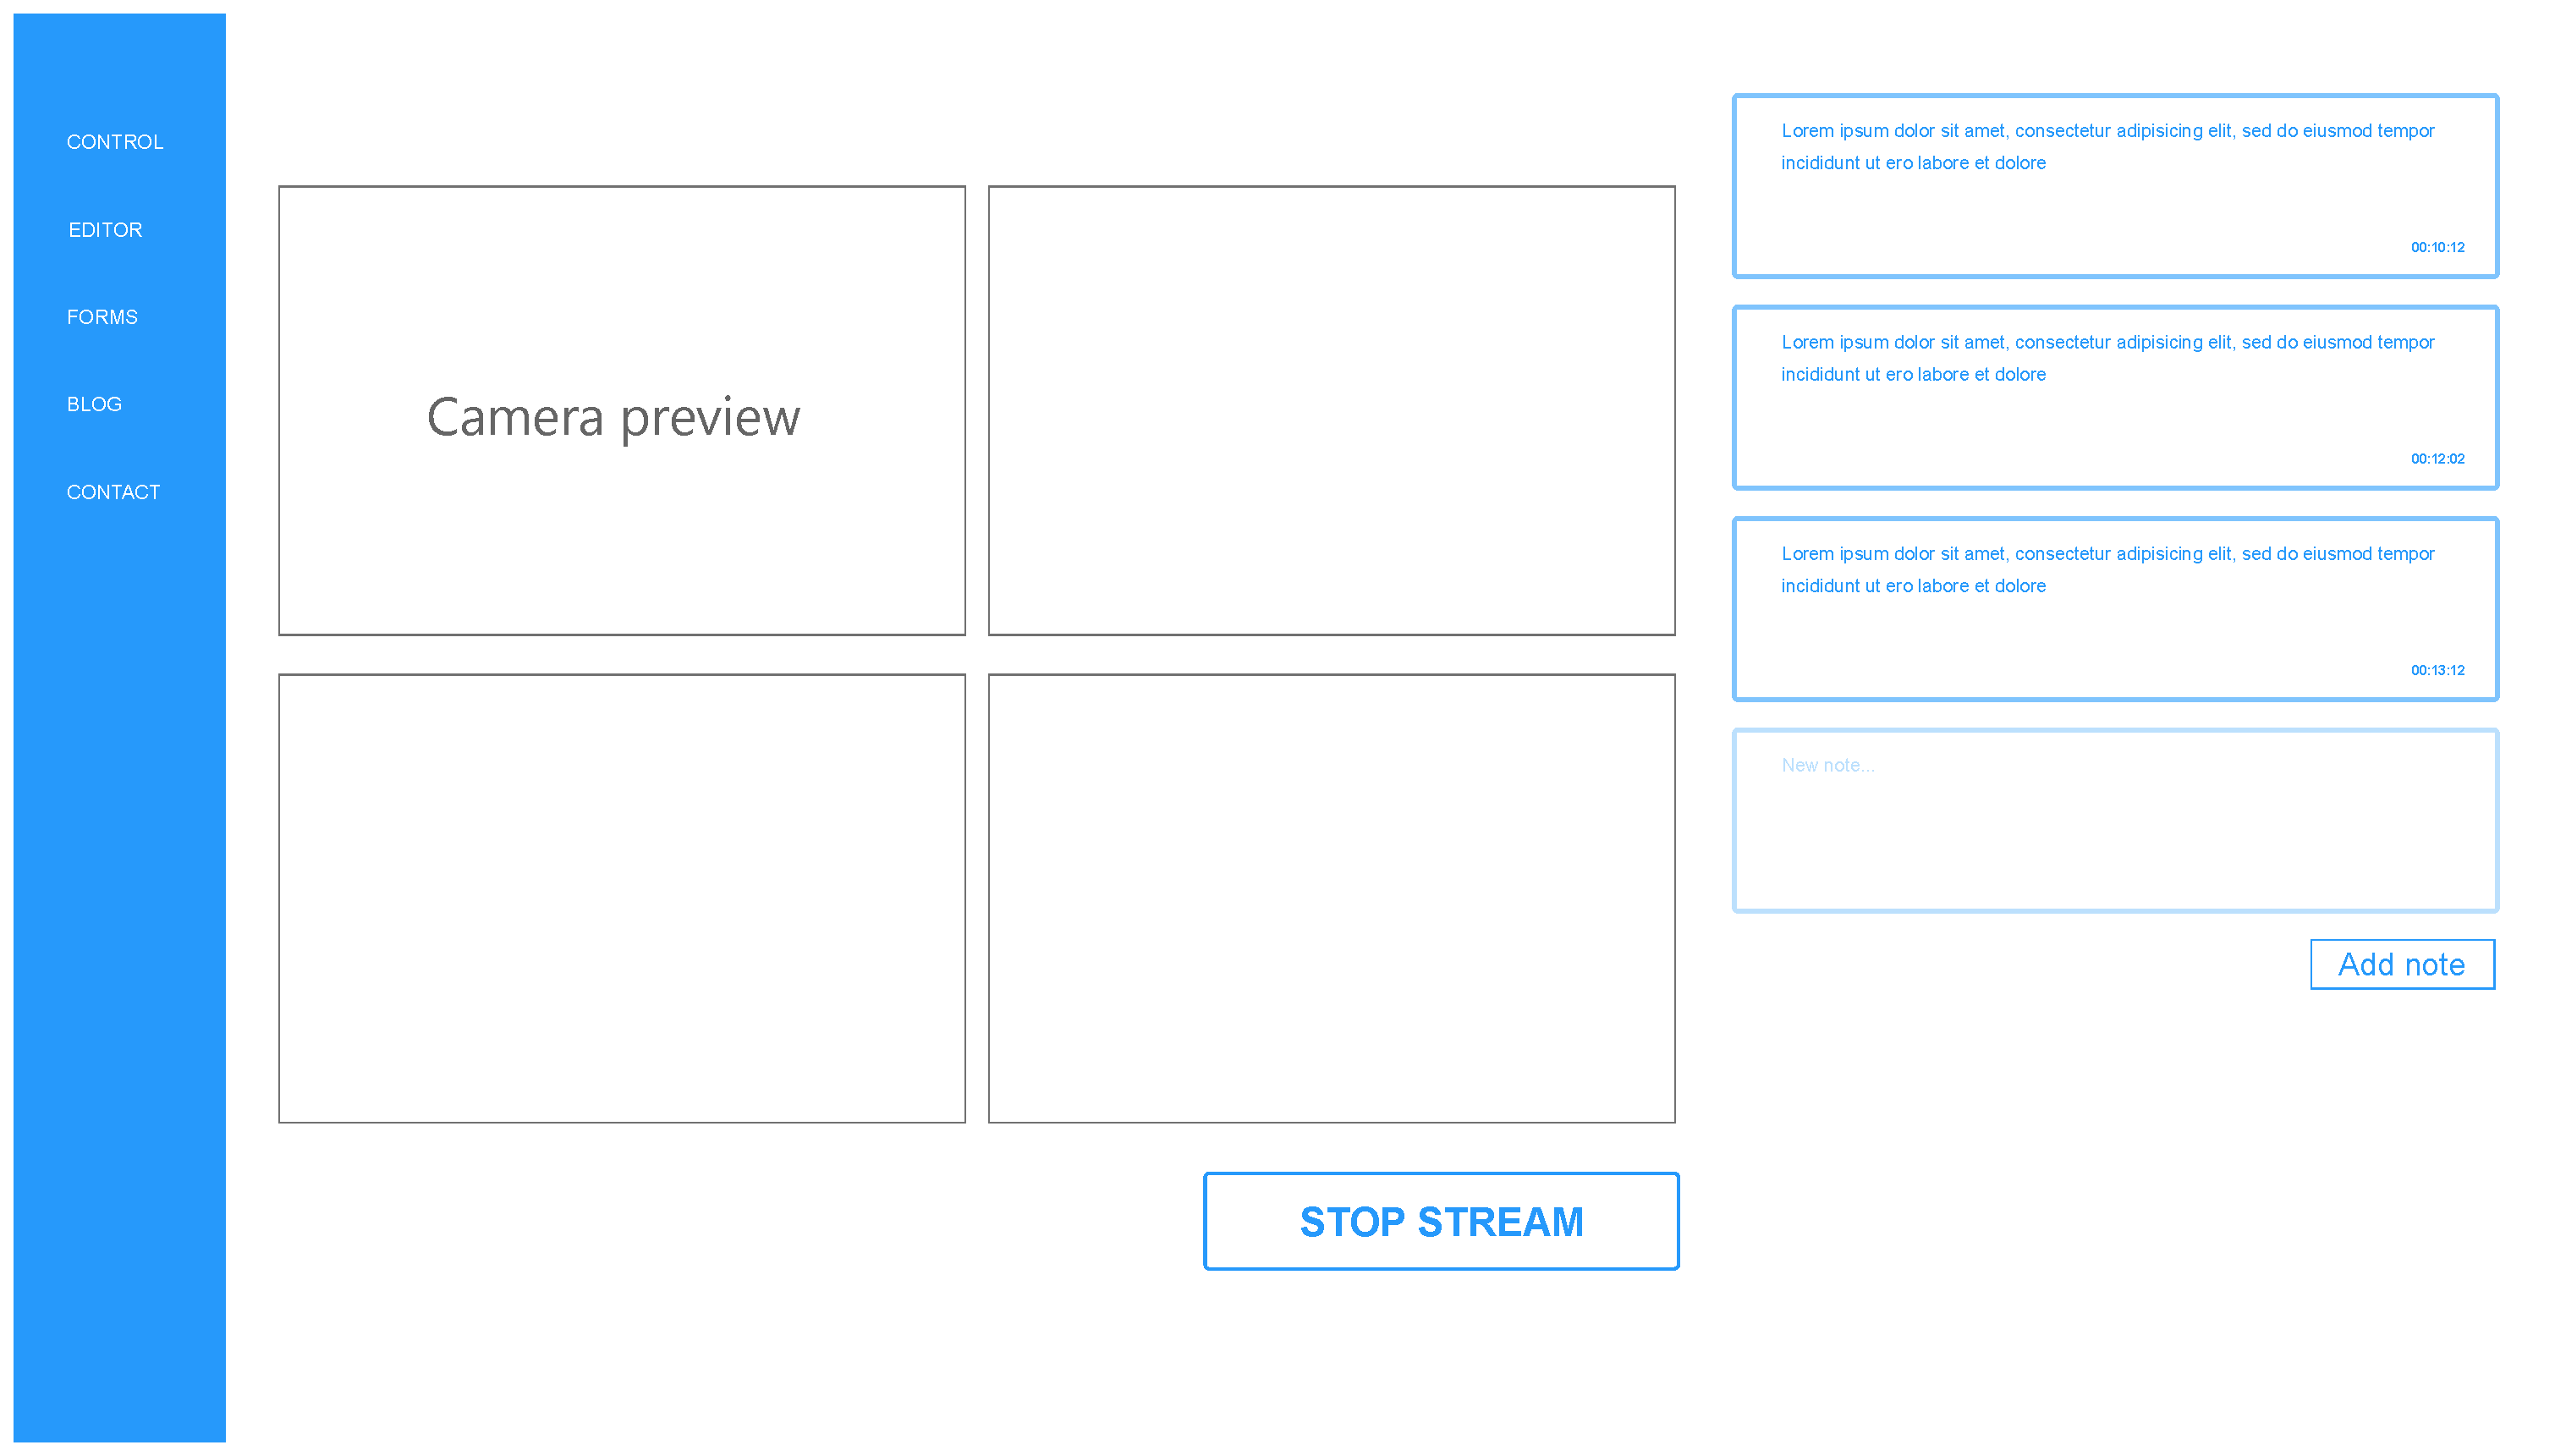
\includegraphics[width=1\textwidth]{images/ui_wf_ulab-stream.eps}
	\caption{Wireframe pro sledování průběhu streamování}\label{img:navrh_frontend_ui_wf_preview}
\end{figure}
\\
\begin{figure}[h]\centering
	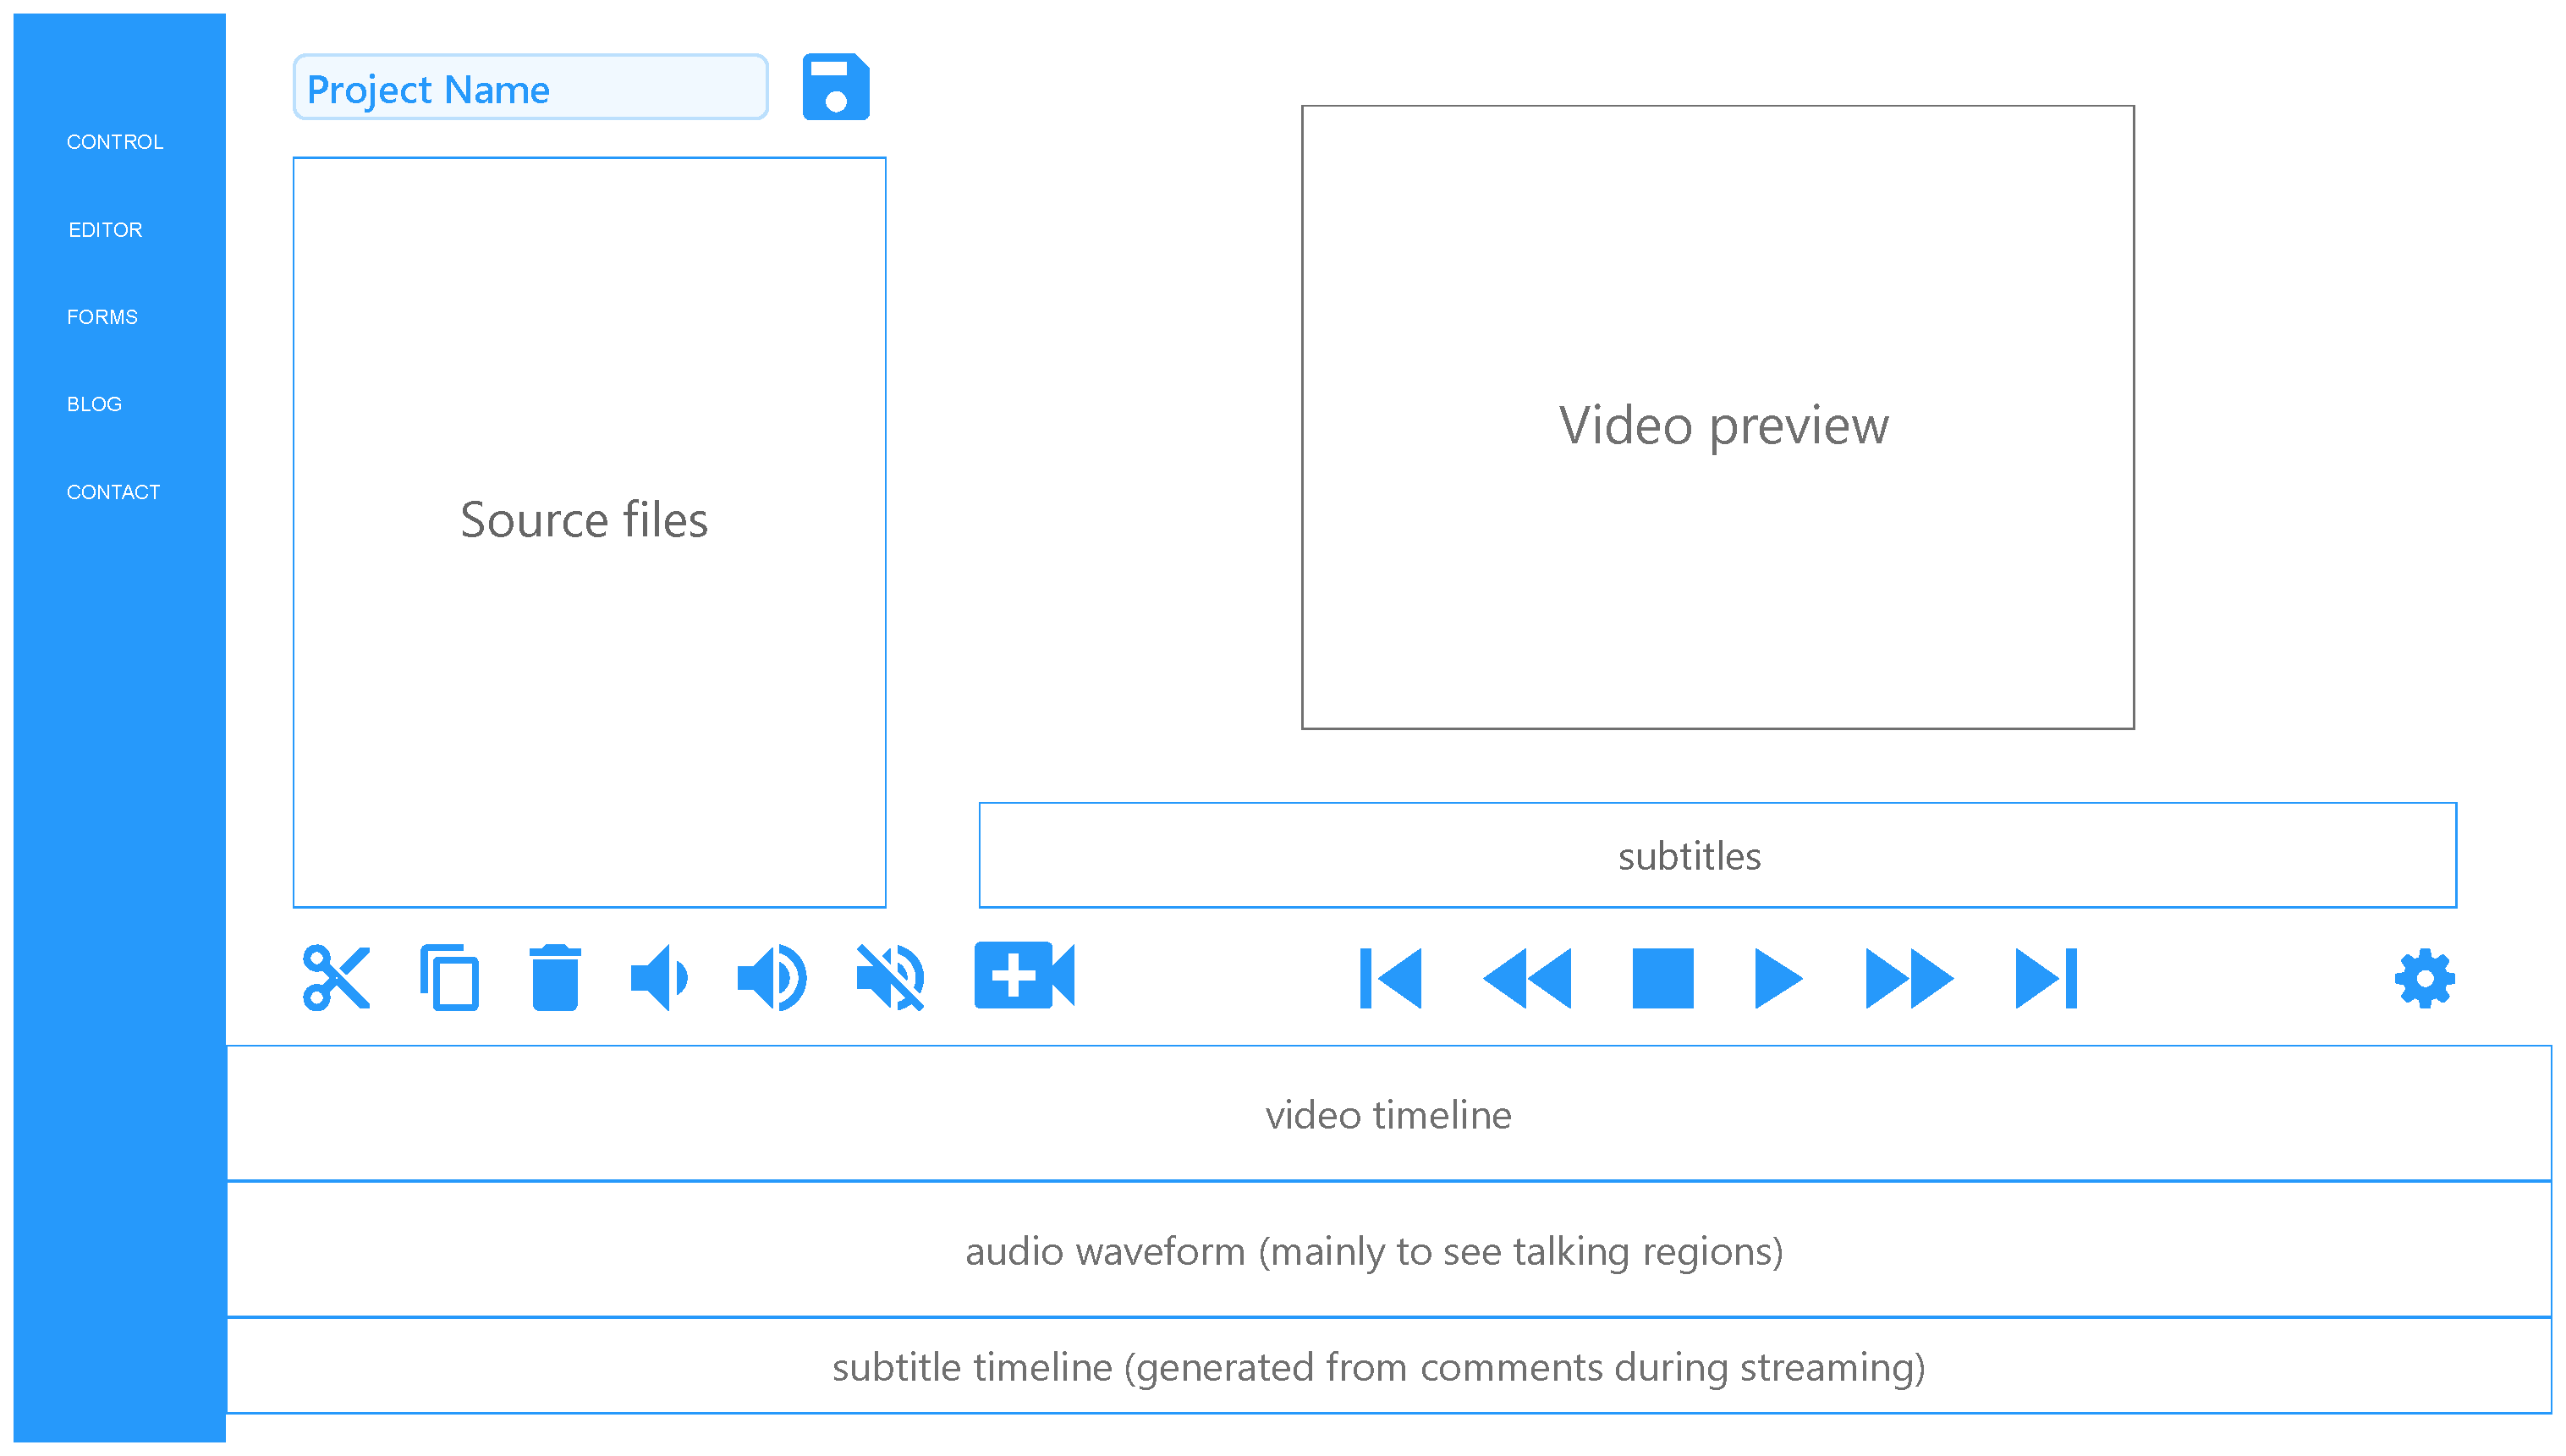
\includegraphics[width=1\textwidth]{images/ui_wf_ulab-editor-1.eps}
	\caption{Wireframe pro videopřehrávač a editor}\label{img:navrh_frontend_ui_wf_editor}
\end{figure}
\\
\begin{figure}[h]\centering
	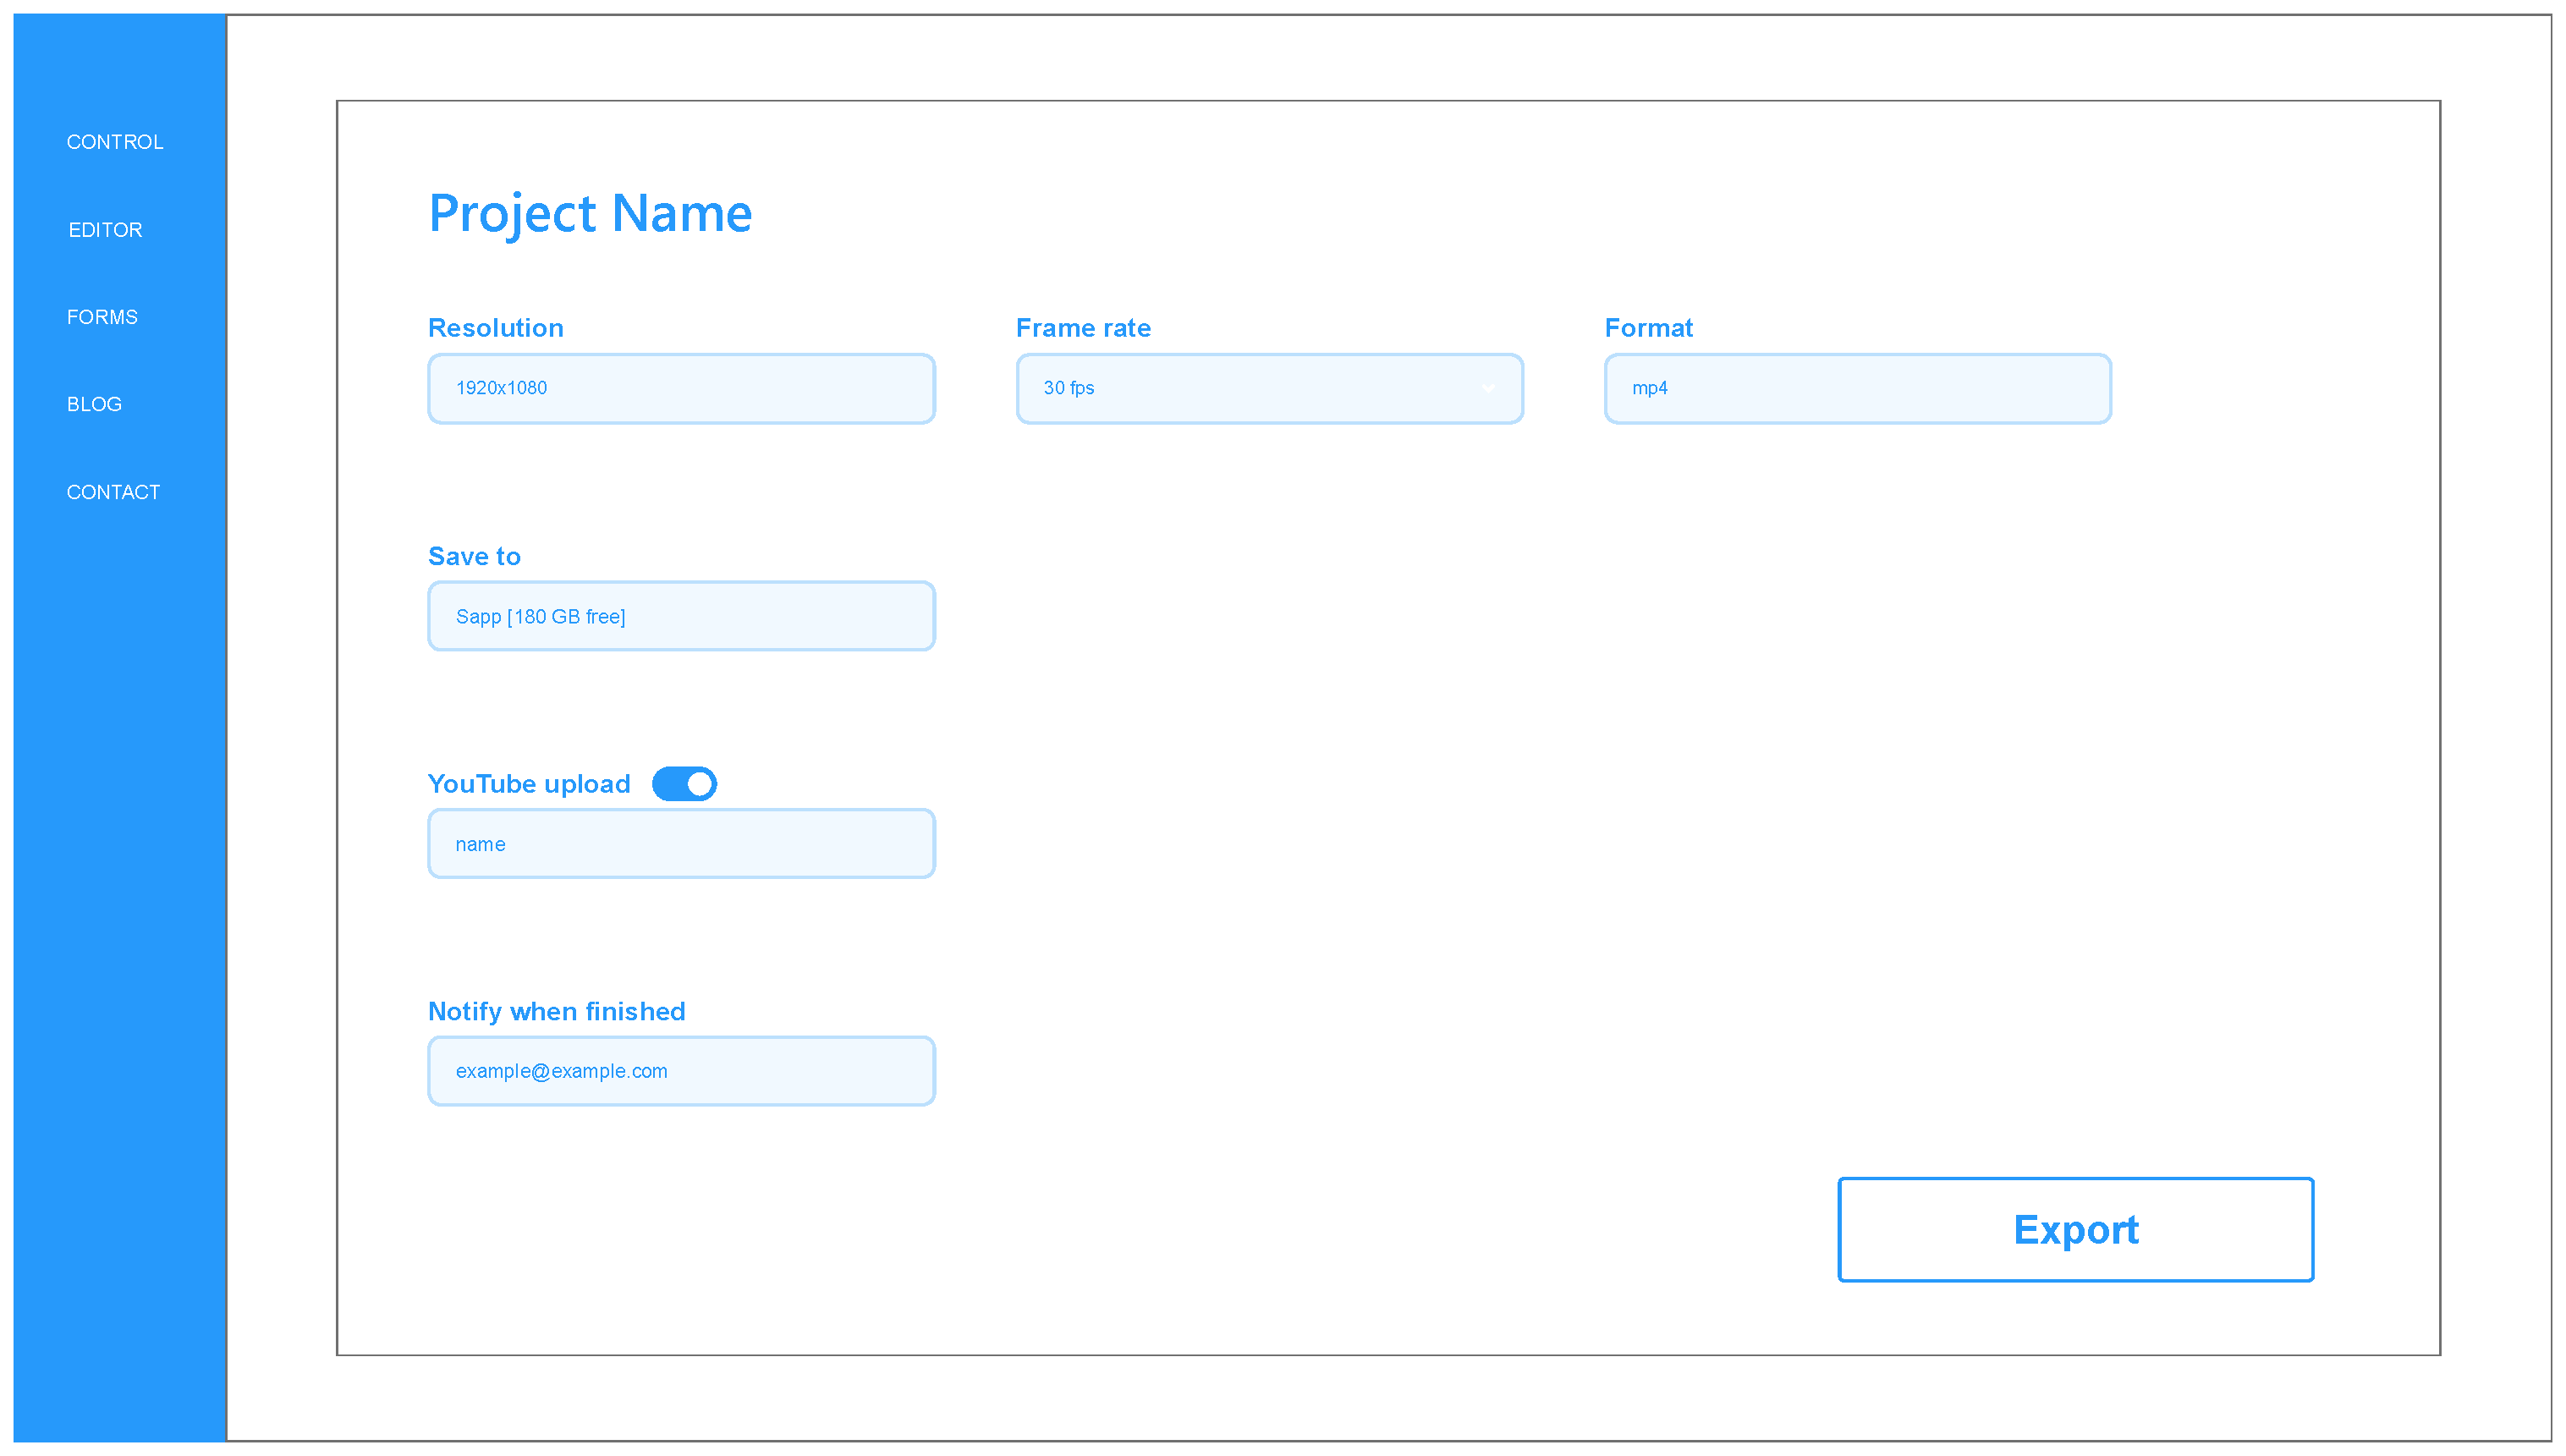
\includegraphics[width=1\textwidth]{images/ui_wf_ulab-editor-export.eps}
	\caption{Wireframe modálního okna pro export}\label{img:navrh_frontend_ui_wf_export}
\end{figure}

\section{Backend} \label{sec:navrh_backend}
\subsection{Databázový model} \label{subsec:navrh_backend_databaze}
Při návrhu relačního databázového modelu se vycházelo z již existujícího modelu. Předchozí práce (\cite{solankar}) totiž již se systémem pro správu videa a streamů částečně počítala ve specifických požadavcích, ale i během vytváření tehdejšího databázového modelu, který již obsahoval tabulku pro videa. Jak bylo zmíněno, tak rozšíření pro správu videí a streamů se v předchozí práci neimplementovalo a tedy i tato funkcionalita byla v databázovém modelu pouze jakýmsi základním prototypem, který bylo nutné řádně poupravit. Na obrázku \ref{img:navrh_backend_db_orig}, který znázorňuje právě databázový model při konci předchozí závěrečné práce, je patrná zmíněná tabulka s videi (\textit{Videos}), která však zdaleka neobsahuje všechny potřebné sloupce.
\\
\begin{figure}[h]\centering
	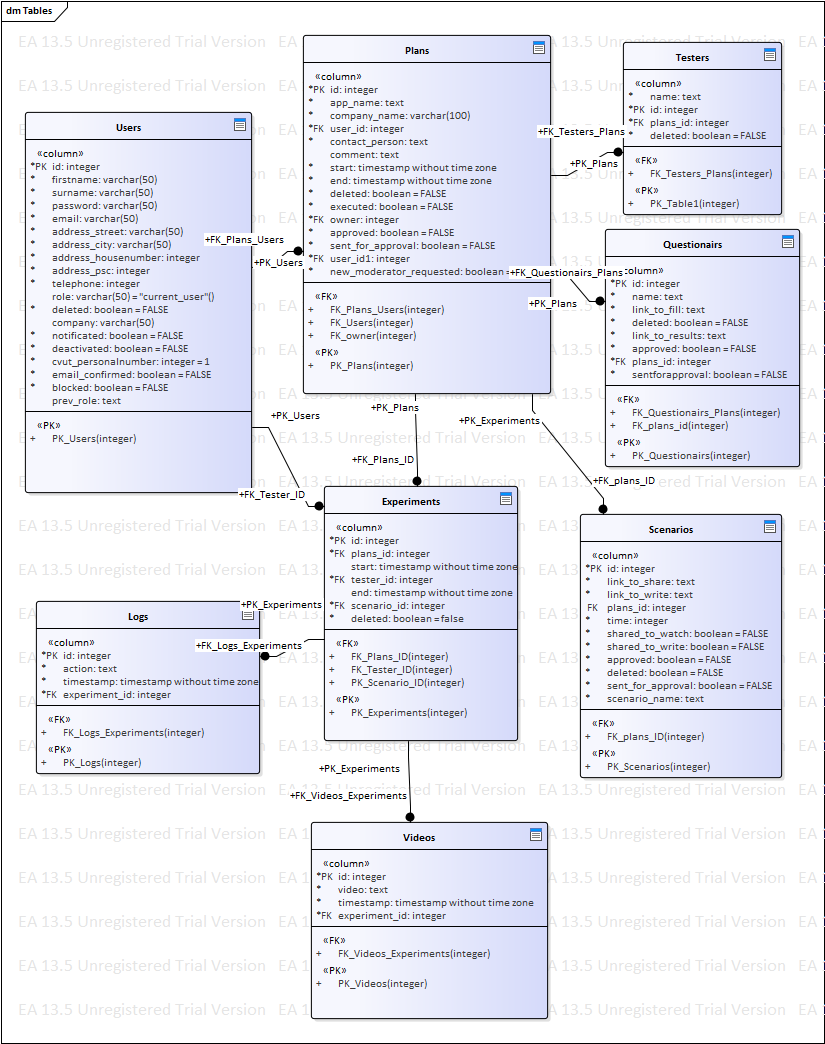
\includegraphics[width=1\textwidth]{images/db_orig.png}
	\caption{Původní databázový model}\label{img:navrh_backend_db_orig}
\end{figure}

Horní část původního databázového modelu (\ref{img:navrh_backend_db_orig}) obsahuje tabulky (např. \textit{Users}, \textit{Logs}, \textit{Plans},...), které se správou videí a streamů příliš nesouvisí, jsou však implementované v původní webové aplikaci a proto jsou zachovány v nezměněné formě novém modelu. Bylo tedy třeba přidat část pro správu videí a informací o nich. Na obrázku \ref{img:navrh_backend_db} je uveden nově vytvořený databázový model, který je pak dále popsán.
\\
\begin{figure}[h]\centering
	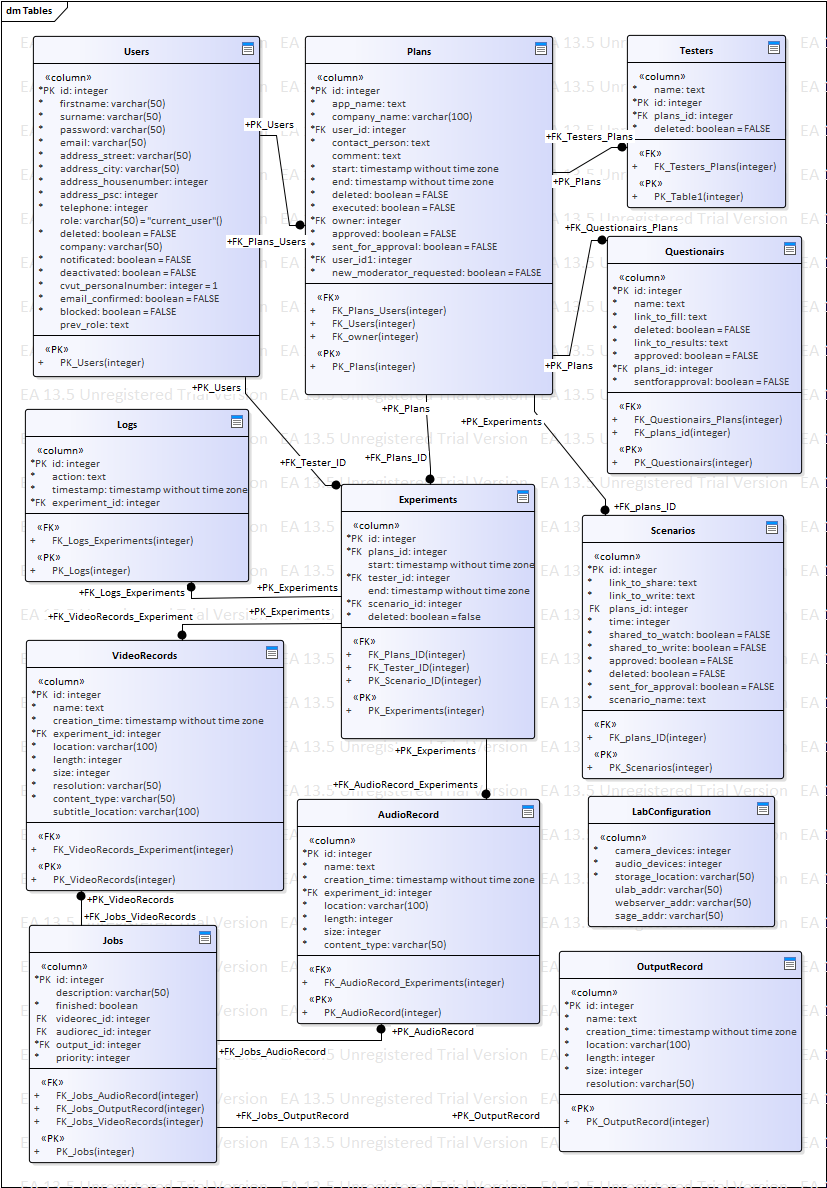
\includegraphics[width=1\textwidth]{images/db.png}
	\caption{Původní databázový model}\label{img:navrh_backend_db}
\end{figure}

Z nového databázového modelu je patrné, že zmizela tabulka s videi a byla nahrazena tabulkou \textit{VideoRecords} a \textit{AudioRecords}. Krom videí bylo také třeba udržovat informace o audio souborech, aby bylo možné s nimi pracovat odděleně (například přidávat a odebírat audio stopy k videu). Z důvodu nemožnosti implementace dědičnosti v relačním databázovém modelu nebyla vytvořena třída \textit{Records}, která by zapouzdřovala možné nahrávky. Dále je z diagramu patrná tabulka \textit{Jobs},  do které se budou ukládat jednotlivé úlohy pro úpravu záznamů (více v sekci \ref{subsec:navrh_backend_ulohy}). Tato tabulka obsahuje vstupní záznamy (relace z tabulek \textit{VideoRecords} a \textit{AudioRecords}), které reprezentují záznamy připravené k nějaké úpravě a dále výstupní záznam realizovaný tabulkou \textit{OutputRecord}. Tabulka \textit{OutputRecord} obsahuje záznamy o médiích vzniklých úpravou jiných po dokončení některé ze zmíněných úloh. Jako poslední je také přidána samostatná tabulka \textit{LabConfiguration}, která obsahuje informace o nahrávacích zařízeních (které jsou připojené a podobně), IP adresy a informace o zařízení SAGE, webserveru, CHUL serveru, úložišti a další.

V tabulkách \textit{VideoRecord}, \textit{AudioRecord}, respektive \textit{OutputRecord} jsou sloupce reprezentující požadované meta-informace nahraných, resp. upravených, záznamů. Veškeré nahrané záznamy se nebudou ukládat do databáze přímo, ale do souborového systému, a databázové tabulky pak budou obsahovat sloupec s lokací, kde se daný záznam v souborovém systému nachází.


\subsection{Správa úloh} \label{subsec:navrh_backend_ulohy}
Při popisování vytvořeného databázového modelu byla zmíněna tabulka \textit{Jobs}, která obsahuje informace o úlohových zpracování záznamů. Dále je popsáno, co za touto tabulkou stojí.

Backendový subsystém pro zpracovávání záznamů upravených ve webové aplikaci je navržen jako dávkové zpracování úloh. V systému se nachází fronta úloh, obsahující úlohy připravené ke zpracování (například převod videa do jiného formátu). Dále je v systému démon, tedy proces běžící na pozadí, který tuto frontu obhospodařuje. Tento proces si hlídá existující zpracovávané úlohy knihovnou Libyuri a pokud se uvolní výpočetní prostředky, pak se z fronty úloh vezme ta s nejvyšší prioritou a začne se zpracovávat. Informace o těchto úlohách jsou uložený právě v tabulce \textit{Jobs}. Na této tabulce je také v PostgreSQL databázi nastavena parametrická notifikace, přesněji příkaz NOTIFY, který, po zápisu nové úlohy do tabulky, notifikuje zmíněného démona pro správu úloh. Tento démon má již na databázi, pomocí příkazu LISTEN, spuštěné naslouchání na kanálu tohoto typu notifikací a za využití PHP funkce \textit{pgsqlGetNotify} pak může vyvolané notifikace zachytávat ve stanovených časových intervalech. Díky tomu dokáže démon vzniklou úlohu zaregistrovat a případně přejít k jejímu zpracování.

\subsection{Libyuri} \label{subsec:navrh_backend_libyuri}
V backendové části aplikace se na CHUL serveru nachází instance knihovny Libyuri. Tato knihovna zde bude sloužit jako prostředník mezi nahrávacími zařízeními v CHUL laboratoři a multimediálním úložištěm, případně webovou aplikací. Reference a návod pro pojmy a různé postupy je k nalezení v analýze v sekci \ref{sec:analyza_yuri}, kde je zevrubně popsáno, jak Libyuri, potažmo aplikace Yuri2 pracuje.	Libyuri na backendu vykonává dva druhy práce jedním je předchozími příkladovými konfiguracemi popsaný proces spouštění nahrávání a streamování a jeho průběh spolu s ukládáním. Další oblastí, při které Libyuri pomůže, bude zpracování videa upraveného ve webovém video editoru. Dále je uveden příklad prvního druhu zmíněné práce Libyri na backendu.

Nejprve je zde, na obrázku \ref{img:navrh_backend_libyuri_sender}, uveden příklad konfigurace Libyuri pro spuštění nahrávání z vybraných zařízení v CHUL laboratoři. Tato konfigurace slouží jednak pro ilustraci toho, které moduly a v jakém pořadí by se měly propojit, a zadruhé jako vzor pro to, jak budou vypadat konfigurace vytvářené za běhu, na základě uživatelova vstupu přes webovou aplikaci. Tato konfigurace se nachází na stroji CHUL server (vizte diagram nasazení \ref{img:navrh_architektura_nasazeni}) při tamní instanci knihovny Libyuri.
\\
\begin{figure}[h]\centering
	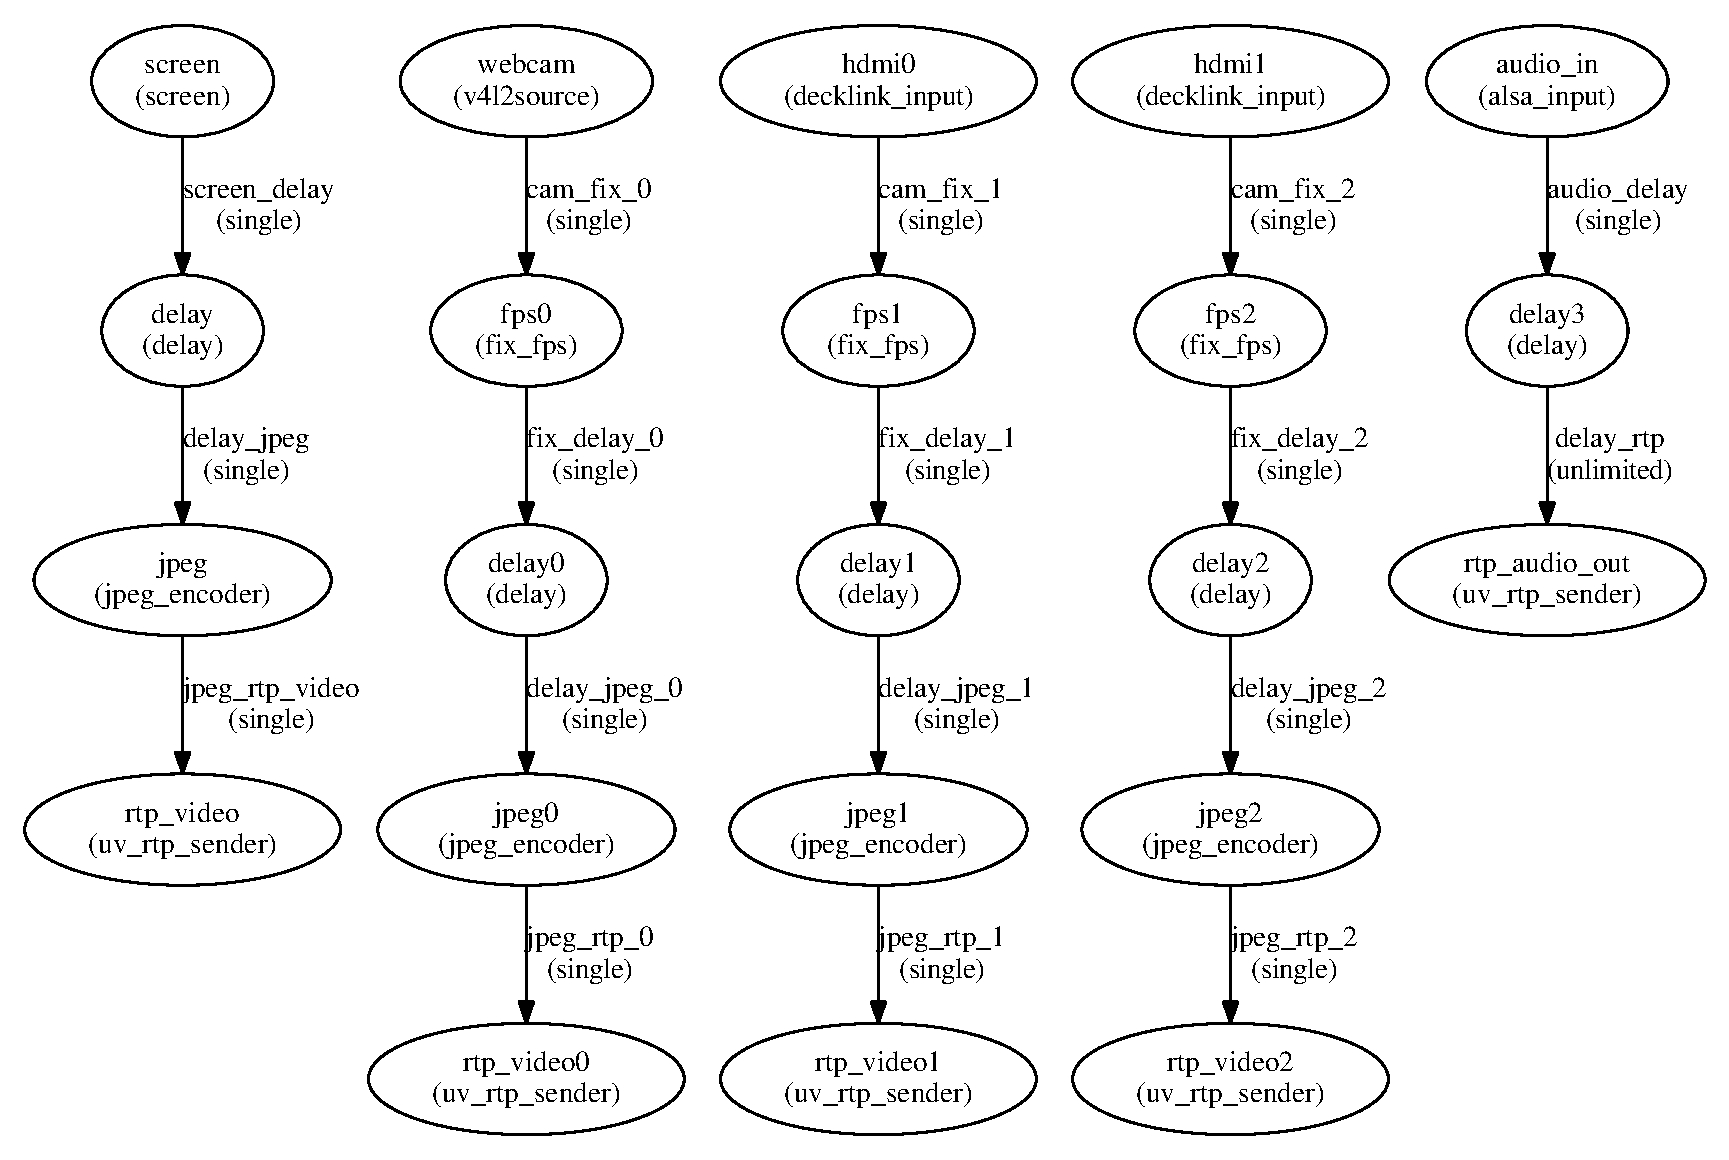
\includegraphics[width=1\textwidth]{images/ulab_sender.eps}
	\caption{Libyuri - konfigurace pro záznam v CHUL}\label{img:navrh_backend_libyuri_sender}
\end{figure}

Uvedený obrázek \ref{img:navrh_backend_libyuri_sender} obsahuje kolečka spojené šipkami, kde každé kolečko reprezentuje uzel a každá šipka reprezentuje orientovanou datovou hranu v grafu konfigurace Libyuri. Každý uzel uvnitř obsahuje svůj název, který je libovolný a pod ním je v závorce přesný název modulu knihovny Libyuri (více v sekci o zpracovávajících uzlech\ref{subsec:analyza_yuri_uzly}), která funkcionalitu tohoto uzlu realizuje, tedy například druhý uzel má název \uv{webcam} a je realizován modulem \uv{v4l2source} (\textit{v4l2} je linuxový ovladač pro práci se zařízeními typu webkamera). Každá orientovaná hrana je popsána obdobným způsobem. Nejprve je uvedeno libovolné jméno hrany a pod ním je v závorce typ datové fronty (více v sekci o datových hranách \ref{subsec:analyza_yuri_hrany}), která jej realizuje (například první hrana shora zleva má název \uv{screen\_delay} a je typu \uv{single}).

V takovéto konfiguraci prezentované obrázkem, který se interpretuje odshora dolů, je patrných pět nahrávacích zařízení, které jsou reprezentovány první řádkou uzlů. Mezi těmito zařízeními jsou zleva: obrazovka počítače (screen), webkamera (webcam), dvě kamery připojené přes rozhraní HDMI (hdmi0 a hdmi1) a nakonec jeden mikrofon (audio\_in). Z kamer putují datové rámce do modulů pro upravení FPS (uzly fps0 -- fps2), dále všechny rámce putují do modulu \textit{delay}, který upraví zpoždění jednotlivých streamů dle potřeby, obrazové streamy pak navštíví modul \textit{jpeg\_encoder} pro kompresi do formátu JPEG čímž se zefektivní přenos dat po síti a nakonec je všech pět streamů modulem \textit{uv\_rtp\_sender} vysláno sítí směrem k cílové IP adrese a portu kde tyto data přebírá jiná instance knihovny Libyuri (například do multimediálního serveru nebo do infrastruktury SAGE). 

Nahrávaná data v laboratoři CHUL a odesílaná po síti pryč by měla být někde přijímána. K tomu slouží další instance knihovny Libyuri s pozměněnou konfigurací pro příjem dat a následné zpracování. Pro ukázku je zde na obrázku \ref{img:navrh_backend_libyuri_receiver} uvedena konfigurace, která se nachází na serveru infrastruktury SAGE, a která přijatá data souběžně ukládá na disk a zároveň streamuje do systému SAGE.
\\
\begin{figure}[h]\centering
	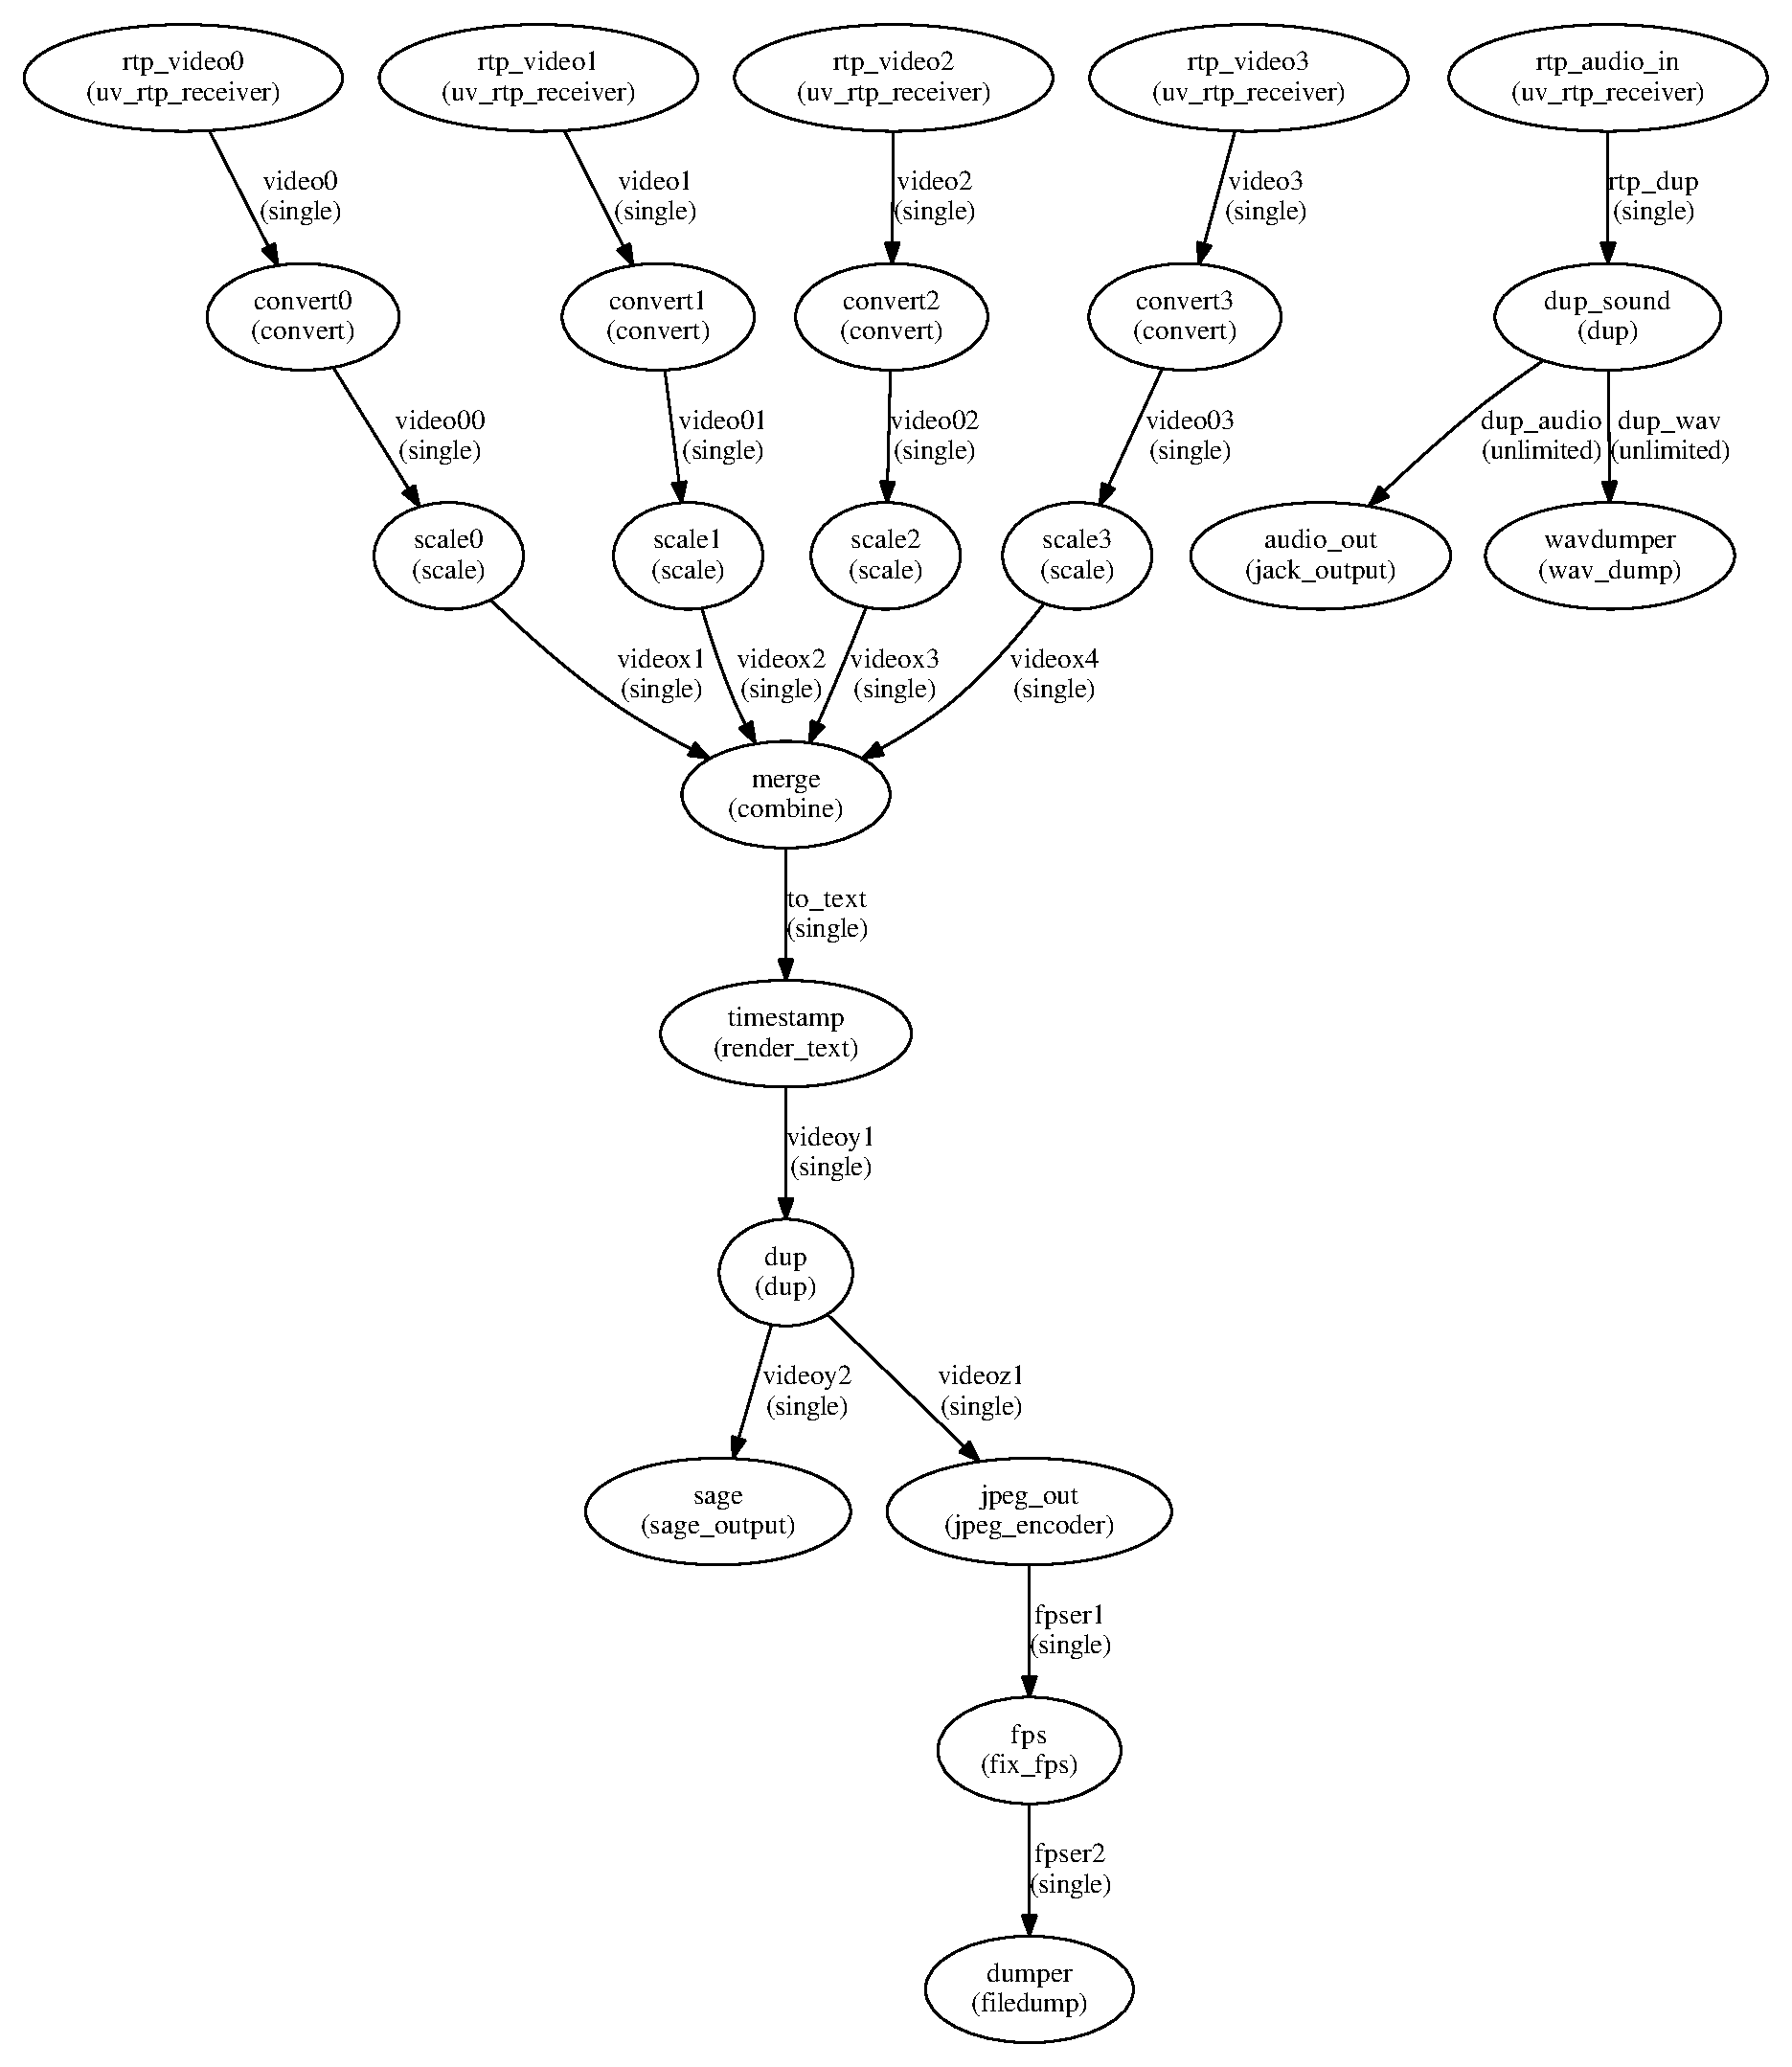
\includegraphics[width=1\textwidth]{images/ulab_receiver.eps}
	\caption{Libyuri - konfigurace zobrazení v SAGE a ukládání}\label{img:navrh_backend_libyuri_receiver}
\end{figure}

Konfigurace na obrázku \ref{img:navrh_backend_libyuri_receiver} má podobnou strukturu, jako předchozí konfigurace. Opět se interpretuje odshora dolů. V první řadě je patrných pět uzlů (uzly rtp\_video0 -- rtp\_video3 a rtp\_audio\_in), které se starají o síťový příjem dat, které byly předchozí konfigurací odesílány pomocí RTP streamů. Obrazová data se ze síťových přijímačů posílají do modulů \textit{convert}, které provedou konverzi obrazů do shodného prostoru barev, dále se pomocí modulu \textit{scale} zmenší či zvětší na požadované rozlišení a všechny se poté spojí vedle sebe do obrazové mřížky v jediném modulu \textit{combine}. Z tohoto modulu dále postupuje pouze jeden stream (který je kombinací všech čtyř obrazových dat) do modulu \textit{render\_text}, který na každý obrazový rámec přidá libovolný text (v tomto případě časovou značku) a nakonec jdou data do modulu \textit{dup}, který stream zduplikuje a jeden z nich pošle do zařízení SAGE (modul \textit{sage\_output}) a druhý po konverzi do formátu JPEG a upravení FPS uloží do souborového systému pomocí modulu \textit{filedump}. Nezmíněná pravá část obrázku \ref{img:navrh_backend_libyuri_receiver}, která zajišťuje zvuková data začíná taktéž uzlem pro příjem RTP streamu. Z něj pak audio data postupují do již zmíněného modulu \textit{dup} a po duplikaci se jeden stream posílá na výstup zvukového zařízení (v tomto případě pomocí modulu \textit{jack\_output}) a druhý se ukládá do souboru modulem \textit{wav\_dump}.


\chapter{Implementace} \label{chap:impl}
Tato kapitola se zabývá implementaci analýzou a návrhem opěvovaného rozšíření stávající aplikace. Nejprve je uvedena sekce o použití systému Gitlab pro verzování aplikace a také pro takzvanou \textit{continuous integration} neboli průběžnou integraci. Dále jsou detailněji popsány některé vybrané implementační zajímavosti. Poté již následuje instalační příručka, ve které je popsáno, jak lze z poskytnutých zdrojových souboru aplikaci nainstalovat do cílového prostředí. V závěru je stručná uživatelská příručka, která prozradí, jak aplikaci používat.

\section{Verzování a continuous integration} \label{sec:impl_gitlab}

\section{Vybrané zajímavé funkce} \label{sec:impl_funkce}

\section{Instalační a uživatelská příručka} \label{sec:impl_prirucka}
TODO .. mozna rozdelit na instalaci a uziv. prirucku



\chapter{Testování} \label{chap:testovani}
\section{Integrační testování} \label{sec:testovani_integracni}	
TODO ... sem dat asi kapku zminku o tetovacim skriptu v CI
\section{Akceptační testování} \label{sec:testovani_akceptacni}
\subsection{Probíhající usability testování} \label{subsec:testovani_akceptacni_utest} % mozna smazat
TODO ... použít něco z NUR - usability testing (prvni prednaska)

\begin{conclusion}
	%sem napište závěr Vaší práce
\end{conclusion}

\nocite{*}
\bibliographystyle{csn690}
\bibliography{mybibliographyfile}

\appendix

\chapter{Seznam použitých zkratek}
% \printglossaries
\begin{description}
	\item[UI] User Interface
	\item[GUI] Graphical User Interface
	\item[API] Application Programming Interface
	\item[XML] eXtensible Markup Language
	\item[HTML] Hypertext Markup Language
\end{description}


% % % % % % % % % % % % % % % % % % % % % % % % % % % % 
% % Tuto kapitolu z výsledné práce ODSTRAŇTE.
% % % % % % % % % % % % % % % % % % % % % % % % % % % % 
% 
% \chapter{Návod k~použití této šablony}
% 
% Tento dokument slouží jako základ pro napsání závěrečné práce na Fakultě informačních technologií ČVUT v~Praze.
% 
% \section{Výběr základu}
% 
% Vyberte si šablonu podle druhu práce (bakalářská, diplomová), jazyka (čeština, angličtina) a kódování (ASCII, \mbox{UTF-8}, \mbox{ISO-8859-2} neboli latin2 a nebo \mbox{Windows-1250}). 
% 
% V~české variantě naleznete šablony v~souborech pojmenovaných ve formátu práce\_kódování.tex. Typ může být:
% \begin{description}
% 	\item[BP] bakalářská práce,
% 	\item[DP] diplomová (magisterská) práce.
% \end{description}
% Kódování, ve kterém chcete psát, může být:
% \begin{description}
% 	\item[UTF-8] kódování Unicode,
% 	\item[ISO-8859-2] latin2,
% 	\item[Windows-1250] znaková sada 1250 Windows.
% \end{description}
% V~případě nejistoty ohledně kódování doporučujeme následující postup:
% \begin{enumerate}
% 	\item Otevřete šablony pro kódování UTF-8 v~editoru prostého textu, který chcete pro psaní práce použít -- pokud můžete texty s~diakritikou normálně přečíst, použijte tuto šablonu.
% 	\item V~opačném případě postupujte dále podle toho, jaký operační systém používáte:
% 	\begin{itemize}
% 		\item v~případě Windows použijte šablonu pro kódování \mbox{Windows-1250},
% 		\item jinak zkuste použít šablonu pro kódování \mbox{ISO-8859-2}.
% 	\end{itemize}
% \end{enumerate}
% 
% 
% V~anglické variantě jsou šablony pojmenované podle typu práce, možnosti jsou:
% \begin{description}
% 	\item[bachelors] bakalářská práce,
% 	\item[masters] diplomová (magisterská) práce.
% \end{description}
% 
% \section{Použití šablony}
% 
% Šablona je určena pro zpracování systémem \LaTeXe{}. Text je možné psát v~textovém editoru jako prostý text, lze však také využít specializovaný editor pro \LaTeX{}, např. Kile.
% 
% Pro získání tisknutelného výstupu z~takto vytvořeného souboru použijte příkaz \verb|pdflatex|, kterému předáte cestu k~souboru jako parametr. Vhodný editor pro \LaTeX{} toto udělá za Vás. \verb|pdfcslatex| ani \verb|cslatex| \emph{nebudou} s~těmito šablonami fungovat.
% 
% Více informací o~použití systému \LaTeX{} najdete např. v~\cite{wikilatex}.
% 
% \subsection{Typografie}
% 
% Při psaní dodržujte typografické konvence zvoleného jazyka. České \uv{uvozovky} zapisujte použitím příkazu \verb|\uv|, kterému v~parametru předáte text, jenž má být v~uvozovkách. Anglické otevírací uvozovky se v~\LaTeX{}u zadávají jako dva zpětné apostrofy, uzavírací uvozovky jako dva apostrofy. Často chybně uváděný symbol "{} (palce) nemá s~uvozovkami nic společného.
% 
% Dále je třeba zabránit zalomení řádky mezi některými slovy, v~češtině např. za jednopísmennými předložkami a spojkami (vyjma \uv{a}). To docílíte vložením pružné nezalomitelné mezery -- znakem \texttt{\textasciitilde}. V~tomto případě to není třeba dělat ručně, lze použít program \verb|vlna|.
% 
% Více o~typografii viz \cite{kobltypo}.
% 
% \subsection{Obrázky}
% 
% Pro umožnění vkládání obrázků je vhodné použít balíček \verb|graphicx|, samotné vložení se provede příkazem \verb|\includegraphics|. Takto je možné vkládat obrázky ve formátu PDF, PNG a JPEG jestliže používáte pdf\LaTeX{} nebo ve formátu EPS jestliže používáte \LaTeX{}. Doporučujeme preferovat vektorové obrázky před rastrovými (vyjma fotografií).
% 
% \subsubsection{Získání vhodného formátu}
% 
% Pro získání vektorových formátů PDF nebo EPS z~jiných lze použít některý z~vektorových grafických editorů. Pro převod rastrového obrázku na vektorový lze použít rasterizaci, kterou mnohé editory zvládají (např. Inkscape). Pro konverze lze použít též nástroje pro dávkové zpracování běžně dodávané s~\LaTeX{}em, např. \verb|epstopdf|.
% 
% \subsubsection{Plovoucí prostředí}
% 
% Příkazem \verb|\includegraphics| lze obrázky vkládat přímo, doporučujeme však použít plovoucí prostředí, konkrétně \verb|figure|. Například obrázek \ref{fig:float} byl vložen tímto způsobem. Vůbec přitom nevadí, když je obrázek umístěn jinde, než bylo původně zamýšleno -- je tomu tak hlavně kvůli dodržení typografických konvencí. Namísto vynucování konkrétní pozice obrázku doporučujeme používat odkazování z~textu (dvojice příkazů \verb|\label| a \verb|\ref|).
% 
% \begin{figure}\centering
% 	
\includegraphics[width=0.5\textwidth, angle=30]{cvut-logo-bw}
% 	\caption[Příklad obrázku]{Ukázkový obrázek v~plovoucím prostředí}\label{fig:float}
% \end{figure}
% 
% \subsubsection{Verze obrázků}
% 
% % Gnuplot BW i barevně
% Může se hodit mít více verzí stejného obrázku, např. pro barevný či černobílý tisk a nebo pro prezentaci. S~pomocí některých nástrojů na generování grafiky je to snadné.
% 
% Máte-li například graf vytvořený v programu Gnuplot, můžete jeho černobílou variantu (viz obr. \ref{fig:gnuplot-bw}) vytvořit parametrem \verb|monochrome dashed| příkazu \verb|set term|. Barevnou variantu (viz obr. \ref{fig:gnuplot-col}) vhodnou na prezentace lze vytvořit parametrem \verb|colour solid|.
% 
% \begin{figure}\centering
% 	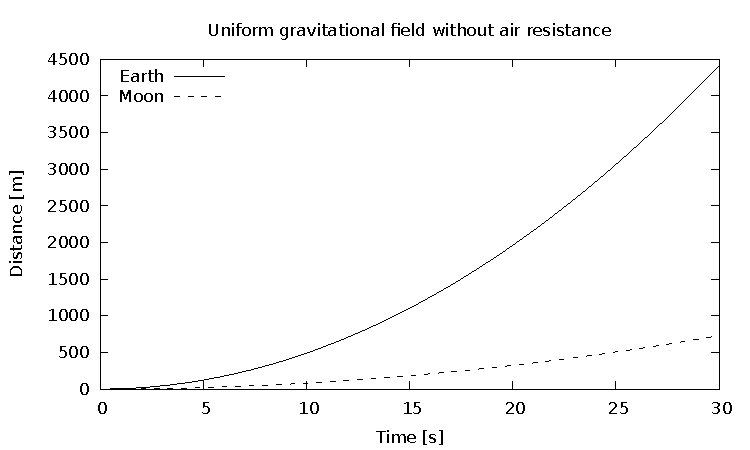
\includegraphics{gnuplot-bw}
% 	\caption{Černobílá varianta obrázku generovaného programem Gnuplot}\label{fig:gnuplot-bw}
% \end{figure}
% 
% \begin{figure}\centering
% 	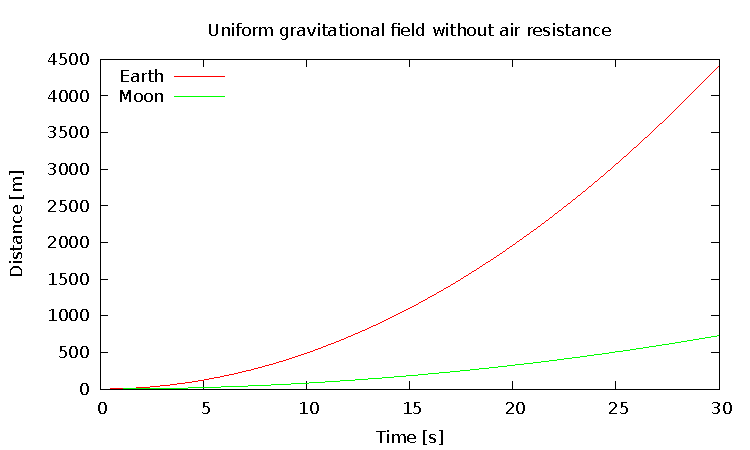
\includegraphics{gnuplot-col}
% 	\caption{Barevná varianta obrázku generovaného programem Gnuplot}\label{fig:gnuplot-col}
% \end{figure}
% 
% 
% \subsection{Tabulky}
% 
% Tabulky lze zadávat různě, např. v~prostředí \verb|tabular|, avšak pro jejich vkládání platí to samé, co pro obrázky -- použijte plovoucí prostředí, v~tomto případě \verb|table|. Například tabulka \ref{tab:matematika} byla vložena tímto způsobem.
% 
% \begin{table}\centering
% 	\caption[Příklad tabulky]{Zadávání matematiky}\label{tab:matematika}
% 	\begin{tabular}{|l|l|c|c|}\hline
% 		Typ		& Prostředí		& \LaTeX{}ovská zkratka	& \TeX{}ovská zkratka	\tabularnewline \hline \hline
% 		Text		& \verb|math|		& \verb|\(...\)|	& \verb|$...$|		\tabularnewline \hline
% 		Displayed	& \verb|displaymath|	& \verb|\[...\]|	& \verb|$$...$$|	\tabularnewline \hline
% 	\end{tabular}
% \end{table}
% 
% % % % % % % % % % % % % % % % % % % % % % % % % % % % 

\chapter{Obsah přiloženého CD}

%upravte podle skutecnosti

\begin{figure}
	\dirtree{%
		.1 readme.txt\DTcomment{stručný popis obsahu CD}.
		.1 exe\DTcomment{adresář se spustitelnou formou implementace}.
		.1 src.
		.2 impl\DTcomment{zdrojové kódy implementace}.
		.2 thesis\DTcomment{zdrojová forma práce ve formátu \LaTeX{}}.
		.1 text\DTcomment{text práce}.
		.2 thesis.pdf\DTcomment{text práce ve formátu PDF}.
		.2 thesis.ps\DTcomment{text práce ve formátu PS}.
	}
\end{figure}

\end{document}
